\documentclass[1p]{elsarticle_modified}
%\bibliographystyle{elsarticle-num}

%\usepackage[colorlinks]{hyperref}
%\usepackage{abbrmath_seonhwa} %\Abb, \Ascr, \Acal ,\Abf, \Afrak
\usepackage{amsfonts}
\usepackage{amssymb}
\usepackage{amsmath}
\usepackage{amsthm}
\usepackage{scalefnt}
\usepackage{amsbsy}
\usepackage{kotex}
\usepackage{caption}
\usepackage{subfig}
\usepackage{color}
\usepackage{graphicx}
\usepackage{xcolor} %% white, black, red, green, blue, cyan, magenta, yellow
\usepackage{float}
\usepackage{setspace}
\usepackage{hyperref}

\usepackage{tikz}
\usetikzlibrary{arrows}

\usepackage{multirow}
\usepackage{array} % fixed length table
\usepackage{hhline}

%%%%%%%%%%%%%%%%%%%%%
\makeatletter
\renewcommand*\env@matrix[1][\arraystretch]{%
	\edef\arraystretch{#1}%
	\hskip -\arraycolsep
	\let\@ifnextchar\new@ifnextchar
	\array{*\c@MaxMatrixCols c}}
\makeatother %https://tex.stackexchange.com/questions/14071/how-can-i-increase-the-line-spacing-in-a-matrix
%%%%%%%%%%%%%%%

\usepackage[normalem]{ulem}

\newcommand{\msout}[1]{\ifmmode\text{\sout{\ensuremath{#1}}}\else\sout{#1}\fi}
%SOURCE: \msout is \stkout macro in https://tex.stackexchange.com/questions/20609/strikeout-in-math-mode

\newcommand{\cancel}[1]{
	\ifmmode
	{\color{red}\msout{#1}}
	\else
	{\color{red}\sout{#1}}
	\fi
}

\newcommand{\add}[1]{
	{\color{blue}\uwave{#1}}
}

\newcommand{\replace}[2]{
	\ifmmode
	{\color{red}\msout{#1}}{\color{blue}\uwave{#2}}
	\else
	{\color{red}\sout{#1}}{\color{blue}\uwave{#2}}
	\fi
}

\newcommand{\Sol}{\mathcal{S}} %segment
\newcommand{\D}{D} %diagram
\newcommand{\A}{\mathcal{A}} %arc


%%%%%%%%%%%%%%%%%%%%%%%%%%%%%5 test

\def\sl{\operatorname{\textup{SL}}(2,\Cbb)}
\def\psl{\operatorname{\textup{PSL}}(2,\Cbb)}
\def\quan{\mkern 1mu \triangleright \mkern 1mu}

\theoremstyle{definition}
\newtheorem{thm}{Theorem}[section]
\newtheorem{prop}[thm]{Proposition}
\newtheorem{lem}[thm]{Lemma}
\newtheorem{ques}[thm]{Question}
\newtheorem{cor}[thm]{Corollary}
\newtheorem{defn}[thm]{Definition}
\newtheorem{exam}[thm]{Example}
\newtheorem{rmk}[thm]{Remark}
\newtheorem{alg}[thm]{Algorithm}

\newcommand{\I}{\sqrt{-1}}
\begin{document}

%\begin{frontmatter}
%
%\title{Boundary parabolic representations of knots up to 8 crossings}
%
%%% Group authors per affiliation:
%\author{Yunhi Cho} 
%\address{Department of Mathematics, University of Seoul, Seoul, Korea}
%\ead{yhcho@uos.ac.kr}
%
%
%\author{Seonhwa Kim} %\fnref{s_kim}}
%\address{Center for Geometry and Physics, Institute for Basic Science, Pohang, 37673, Korea}
%\ead{ryeona17@ibs.re.kr}
%
%\author{Hyuk Kim}
%\address{Department of Mathematical Sciences, Seoul National University, Seoul 08826, Korea}
%\ead{hyukkim@snu.ac.kr}
%
%\author{Seokbeom Yoon}
%\address{Department of Mathematical Sciences, Seoul National University, Seoul, 08826,  Korea}
%\ead{sbyoon15@snu.ac.kr}
%
%\begin{abstract}
%We find all boundary parabolic representation of knots up to 8 crossings.
%
%\end{abstract}
%\begin{keyword}
%    \MSC[2010] 57M25 
%\end{keyword}
%
%\end{frontmatter}

%\linenumbers
%\tableofcontents
%
\newcommand\colored[1]{\textcolor{white}{\rule[-0.35ex]{0.8em}{1.4ex}}\kern-0.8em\color{red} #1}%
%\newcommand\colored[1]{\textcolor{white}{ #1}\kern-2.17ex	\textcolor{white}{ #1}\kern-1.81ex	\textcolor{white}{ #1}\kern-2.15ex\color{red}#1	}

{\Large $\underline{12a_{0701}~(K12a_{0701})}$}

\setlength{\tabcolsep}{10pt}
\renewcommand{\arraystretch}{1.6}
\vspace{1cm}\begin{tabular}{m{100pt}>{\centering\arraybackslash}m{274pt}}
\multirow{5}{120pt}{
	\centering
	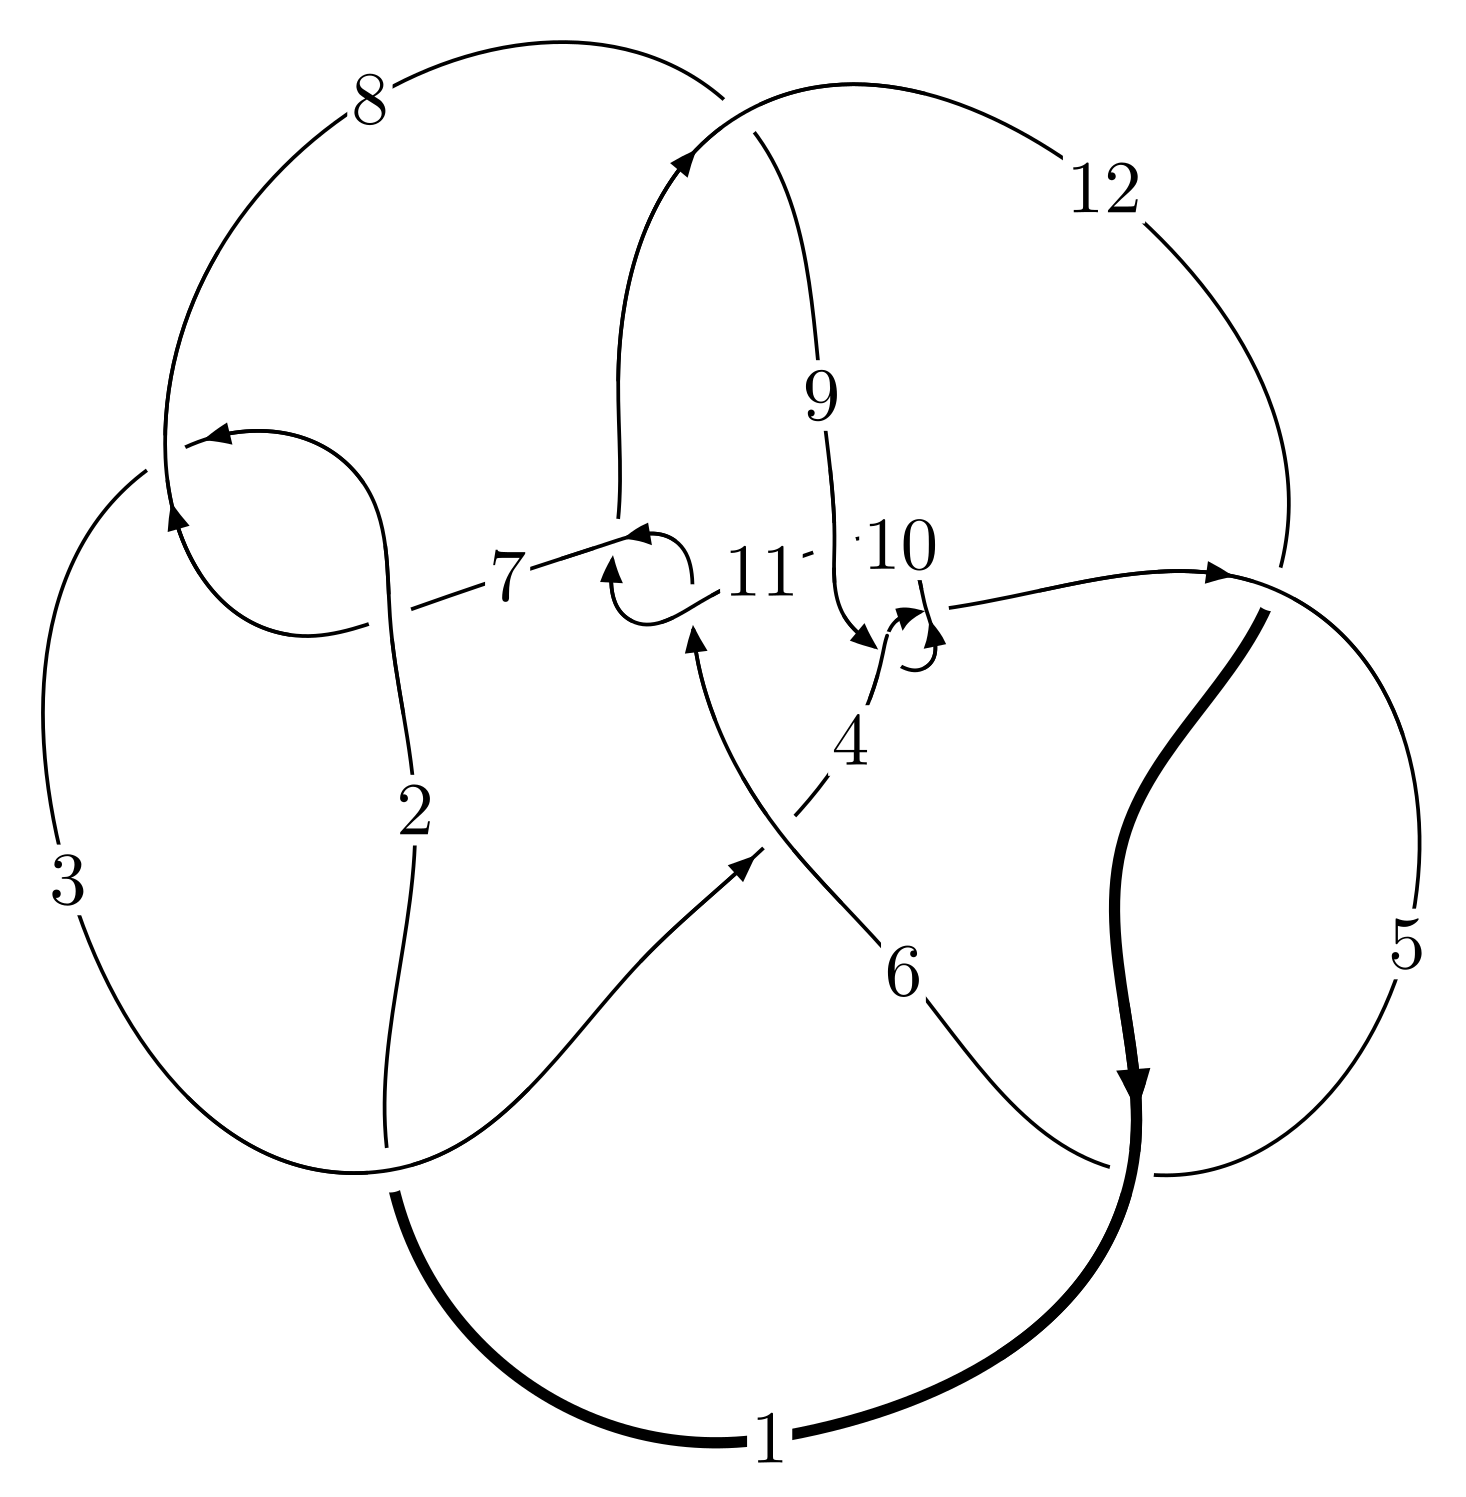
\includegraphics[width=112pt]{../../../GIT/diagram.site/diagram/png/1502_12a_0701.png}\\
\ \ \ A knot diagram\footnotemark}&
\allowdisplaybreaks
\textbf{Linearized knot diagam} \\
\cline{2-2}
 &
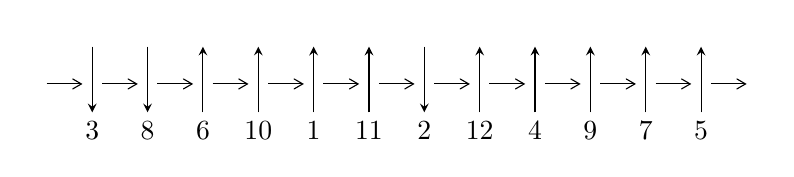
\begin{tikzpicture}[x=20pt, y=17pt]
	% nodes
	\node (C0) at (0, 0) {};
	\node (C1) at (1, 0) {};
	\node (C1U) at (1, +1) {};
	\node (C1D) at (1, -1) {3};

	\node (C2) at (2, 0) {};
	\node (C2U) at (2, +1) {};
	\node (C2D) at (2, -1) {8};

	\node (C3) at (3, 0) {};
	\node (C3U) at (3, +1) {};
	\node (C3D) at (3, -1) {6};

	\node (C4) at (4, 0) {};
	\node (C4U) at (4, +1) {};
	\node (C4D) at (4, -1) {10};

	\node (C5) at (5, 0) {};
	\node (C5U) at (5, +1) {};
	\node (C5D) at (5, -1) {1};

	\node (C6) at (6, 0) {};
	\node (C6U) at (6, +1) {};
	\node (C6D) at (6, -1) {11};

	\node (C7) at (7, 0) {};
	\node (C7U) at (7, +1) {};
	\node (C7D) at (7, -1) {2};

	\node (C8) at (8, 0) {};
	\node (C8U) at (8, +1) {};
	\node (C8D) at (8, -1) {12};

	\node (C9) at (9, 0) {};
	\node (C9U) at (9, +1) {};
	\node (C9D) at (9, -1) {4};

	\node (C10) at (10, 0) {};
	\node (C10U) at (10, +1) {};
	\node (C10D) at (10, -1) {9};

	\node (C11) at (11, 0) {};
	\node (C11U) at (11, +1) {};
	\node (C11D) at (11, -1) {7};

	\node (C12) at (12, 0) {};
	\node (C12U) at (12, +1) {};
	\node (C12D) at (12, -1) {5};
	\node (C13) at (13, 0) {};

	% arrows
	\draw[->,>={angle 60}]
	(C0) edge (C1) (C1) edge (C2) (C2) edge (C3) (C3) edge (C4) (C4) edge (C5) (C5) edge (C6) (C6) edge (C7) (C7) edge (C8) (C8) edge (C9) (C9) edge (C10) (C10) edge (C11) (C11) edge (C12) (C12) edge (C13) ;	\draw[->,>=stealth]
	(C1U) edge (C1D) (C2U) edge (C2D) (C3D) edge (C3U) (C4D) edge (C4U) (C5D) edge (C5U) (C6D) edge (C6U) (C7U) edge (C7D) (C8D) edge (C8U) (C9D) edge (C9U) (C10D) edge (C10U) (C11D) edge (C11U) (C12D) edge (C12U) ;
	\end{tikzpicture} \\
\hhline{~~} \\& 
\textbf{Solving Sequence} \\ \cline{2-2} 
 &
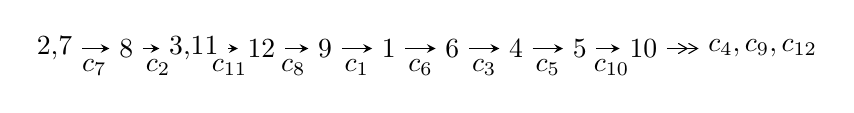
\begin{tikzpicture}[x=23pt, y=7pt]
	% node
	\node (A0) at (-1/8, 0) {2,7};
	\node (A1) at (1, 0) {8};
	\node (A2) at (33/16, 0) {3,11};
	\node (A3) at (25/8, 0) {12};
	\node (A4) at (33/8, 0) {9};
	\node (A5) at (41/8, 0) {1};
	\node (A6) at (49/8, 0) {6};
	\node (A7) at (57/8, 0) {4};
	\node (A8) at (65/8, 0) {5};
	\node (A9) at (73/8, 0) {10};
	\node (C1) at (1/2, -1) {$c_{7}$};
	\node (C2) at (3/2, -1) {$c_{2}$};
	\node (C3) at (21/8, -1) {$c_{11}$};
	\node (C4) at (29/8, -1) {$c_{8}$};
	\node (C5) at (37/8, -1) {$c_{1}$};
	\node (C6) at (45/8, -1) {$c_{6}$};
	\node (C7) at (53/8, -1) {$c_{3}$};
	\node (C8) at (61/8, -1) {$c_{5}$};
	\node (C9) at (69/8, -1) {$c_{10}$};
	\node (A10) at (11, 0) {$c_{4},c_{9},c_{12}$};

	% edge
	\draw[->,>=stealth]	
	(A0) edge (A1) (A1) edge (A2) (A2) edge (A3) (A3) edge (A4) (A4) edge (A5) (A5) edge (A6) (A6) edge (A7) (A7) edge (A8) (A8) edge (A9) ;
	\draw[->>,>={angle 60}]	
	(A9) edge (A10);
\end{tikzpicture} \\ 

\end{tabular} \\

\footnotetext{
The image of knot diagram is generated by the software ``\textbf{Draw programme}" developed by Andrew Bartholomew(\url{http://www.layer8.co.uk/maths/draw/index.htm\#Running-draw}), where we modified some parts for our purpose(\url{https://github.com/CATsTAILs/LinksPainter}).
}\phantom \\ \newline 
\centering \textbf{Ideals for irreducible components\footnotemark of $X_{\text{par}}$} 
 
\begin{align*}
I^u_{1}&=\langle 
-7.70053\times10^{53} u^{39}-1.74213\times10^{54} u^{38}+\cdots+2.50493\times10^{54} b-1.01102\times10^{54},\\
\phantom{I^u_{1}}&\phantom{= \langle  }5.17594\times10^{54} u^{39}+1.38121\times10^{55} u^{38}+\cdots+1.08547\times10^{55} a-8.78741\times10^{53},\\
\phantom{I^u_{1}}&\phantom{= \langle  }5 u^{40}+15 u^{39}+\cdots+4 u+13\rangle \\
I^u_{2}&=\langle 
2 u^{31} a+3 u^{31}+\cdots-2 a+4,\;2 u^{30} a+16 u^{31}+\cdots+2 a-15,\;u^{32}- u^{31}+\cdots-2 u+1\rangle \\
I^u_{3}&=\langle 
- u^3+b,\;u^3+u^2+2 a-2 u,\;u^4- u^2+1\rangle \\
I^u_{4}&=\langle 
b,\;a-1,\;u^4- u^3+1\rangle \\
I^u_{5}&=\langle 
b+1,\;- u^3+a-1,\;u^4- u^3+1\rangle \\
I^u_{6}&=\langle 
b,\;a-1,\;u+1\rangle \\
I^u_{7}&=\langle 
b+1,\;a,\;u+1\rangle \\
I^u_{8}&=\langle 
- u^3+b,\;u^3+2 a-2 u-1,\;u^4- u^2+1\rangle \\
I^u_{9}&=\langle 
b+1,\;u^5 a- u^5- u^3 a+2 u^3+a u- u+1\rangle \\
\\
\end{align*}
\raggedright * 8 irreducible components of $\dim_{\mathbb{C}}=0$, with total 122 representations.\\
\raggedright * 1 irreducible components of $\dim_{\mathbb{C}}=1$ \\
\footnotetext{All coefficients of polynomials are rational numbers. But the coefficients are sometimes approximated in decimal forms when there is not enough margin.}
\newpage
\renewcommand{\arraystretch}{1}
\centering \section*{I. $I^u_{1}= \langle -7.70\times10^{53} u^{39}-1.74\times10^{54} u^{38}+\cdots+2.50\times10^{54} b-1.01\times10^{54},\;5.18\times10^{54} u^{39}+1.38\times10^{55} u^{38}+\cdots+1.09\times10^{55} a-8.79\times10^{53},\;5 u^{40}+15 u^{39}+\cdots+4 u+13 \rangle$}
\flushleft \textbf{(i) Arc colorings}\\
\begin{tabular}{m{7pt} m{180pt} m{7pt} m{180pt} }
\flushright $a_{2}=$&$\begin{pmatrix}0\\u\end{pmatrix}$ \\
\flushright $a_{7}=$&$\begin{pmatrix}1\\0\end{pmatrix}$ \\
\flushright $a_{8}=$&$\begin{pmatrix}1\\u^2\end{pmatrix}$ \\
\flushright $a_{3}=$&$\begin{pmatrix}- u\\- u^3+u\end{pmatrix}$ \\
\flushright $a_{11}=$&$\begin{pmatrix}-0.476839 u^{39}-1.27246 u^{38}+\cdots-5.39284 u+0.0809549\\0.307415 u^{39}+0.695481 u^{38}+\cdots+2.07333 u+0.403613\end{pmatrix}$ \\
\flushright $a_{12}=$&$\begin{pmatrix}-0.169424 u^{39}-0.576975 u^{38}+\cdots-3.31951 u+0.484568\\0.307415 u^{39}+0.695481 u^{38}+\cdots+2.07333 u+0.403613\end{pmatrix}$ \\
\flushright $a_{9}=$&$\begin{pmatrix}-0.211994 u^{39}-0.480895 u^{38}+\cdots-3.96053 u-0.213115\\0.0500582 u^{39}+0.116432 u^{38}+\cdots+0.995645 u+0.307144\end{pmatrix}$ \\
\flushright $a_{1}=$&$\begin{pmatrix}u^3\\u^5- u^3+u\end{pmatrix}$ \\
\flushright $a_{6}=$&$\begin{pmatrix}-0.191581 u^{39}-0.280282 u^{38}+\cdots+5.99057 u+1.63083\\-0.0736869 u^{39}-0.292199 u^{38}+\cdots-0.484607 u-0.887781\end{pmatrix}$ \\
\flushright $a_{4}=$&$\begin{pmatrix}0.231719 u^{39}+0.602871 u^{38}+\cdots+1.98498 u-0.495273\\0.0632015 u^{39}+0.154197 u^{38}+\cdots+0.0133278 u+0.385259\end{pmatrix}$ \\
\flushright $a_{5}=$&$\begin{pmatrix}-0.245279 u^{39}-0.480339 u^{38}+\cdots+6.44253 u+1.18353\\-0.133010 u^{39}-0.382392 u^{38}+\cdots-0.608099 u-1.13846\end{pmatrix}$ \\
\flushright $a_{10}=$&$\begin{pmatrix}-0.660060 u^{39}-1.59385 u^{38}+\cdots-8.11569 u-0.968106\\0.246464 u^{39}+0.516908 u^{38}+\cdots+1.74196 u+0.398054\end{pmatrix}$\\&\end{tabular}
\flushleft \textbf{(ii) Obstruction class $= -1$}\\~\\
\flushleft \textbf{(iii) Cusp Shapes $= 0.355272 u^{39}+2.47238 u^{38}+\cdots+1.40321 u+8.32948$}\\~\\
\newpage\renewcommand{\arraystretch}{1}
\flushleft \textbf{(iv) u-Polynomials at the component}\newline \\
\begin{tabular}{m{50pt}|m{274pt}}
Crossings & \hspace{64pt}u-Polynomials at each crossing \\
\hline $$\begin{aligned}c_{1}\end{aligned}$$&$\begin{aligned}
&25(25 u^{40}+355 u^{39}+\cdots-2766 u+169)
\end{aligned}$\\
\hline $$\begin{aligned}c_{2},c_{7}\end{aligned}$$&$\begin{aligned}
&5(5 u^{40}-15 u^{39}+\cdots-4 u+13)
\end{aligned}$\\
\hline $$\begin{aligned}c_{3},c_{8}\end{aligned}$$&$\begin{aligned}
&64(64 u^{40}+192 u^{39}+\cdots+80 u+25)
\end{aligned}$\\
\hline $$\begin{aligned}c_{4},c_{9}\end{aligned}$$&$\begin{aligned}
&5(5 u^{40}-15 u^{39}+\cdots-58 u+13)
\end{aligned}$\\
\hline $$\begin{aligned}c_{5},c_{6},c_{11}\\c_{12}\end{aligned}$$&$\begin{aligned}
&u^{40}+4 u^{39}+\cdots+36 u+4
\end{aligned}$\\
\hline $$\begin{aligned}c_{10}\end{aligned}$$&$\begin{aligned}
&25(25 u^{40}-455 u^{39}+\cdots+718 u+169)
\end{aligned}$\\
\hline
\end{tabular}\\~\\
\newpage\renewcommand{\arraystretch}{1}
\flushleft \textbf{(v) Riley Polynomials at the component}\newline \\
\begin{tabular}{m{50pt}|m{274pt}}
Crossings & \hspace{64pt}Riley Polynomials at each crossing \\
\hline $$\begin{aligned}c_{1}\end{aligned}$$&$\begin{aligned}
&625(625 y^{40}+14425 y^{39}+\cdots-2166706 y+28561)
\end{aligned}$\\
\hline $$\begin{aligned}c_{2},c_{7}\end{aligned}$$&$\begin{aligned}
&25(25 y^{40}-355 y^{39}+\cdots+2766 y+169)
\end{aligned}$\\
\hline $$\begin{aligned}c_{3},c_{8}\end{aligned}$$&$\begin{aligned}
&4096(4096 y^{40}-53248 y^{39}+\cdots-13450 y+625)
\end{aligned}$\\
\hline $$\begin{aligned}c_{4},c_{9}\end{aligned}$$&$\begin{aligned}
&25(25 y^{40}-455 y^{39}+\cdots+718 y+169)
\end{aligned}$\\
\hline $$\begin{aligned}c_{5},c_{6},c_{11}\\c_{12}\end{aligned}$$&$\begin{aligned}
&y^{40}-12 y^{39}+\cdots-696 y+16
\end{aligned}$\\
\hline $$\begin{aligned}c_{10}\end{aligned}$$&$\begin{aligned}
&625(625 y^{40}+4425 y^{39}+\cdots-2689202 y+28561)
\end{aligned}$\\
\hline
\end{tabular}\\~\\
\newpage\flushleft \textbf{(vi) Complex Volumes and Cusp Shapes}
$$\begin{array}{c|c|c}  
\text{Solutions to }I^u_{1}& \I (\text{vol} + \sqrt{-1}CS) & \text{Cusp shape}\\
 \hline 
\begin{aligned}
u &= -0.970531 + 0.178964 I \\
a &= -0.833678 + 1.090430 I \\
b &= \phantom{-}0.657380 + 0.842879 I\end{aligned}
 & -4.36949 + 3.79276 I & -0.84937 - 5.47947 I \\ \hline\begin{aligned}
u &= -0.970531 - 0.178964 I \\
a &= -0.833678 - 1.090430 I \\
b &= \phantom{-}0.657380 - 0.842879 I\end{aligned}
 & -4.36949 - 3.79276 I & -0.84937 + 5.47947 I \\ \hline\begin{aligned}
u &= -0.800492 + 0.625954 I \\
a &= -1.186250 - 0.317798 I \\
b &= \phantom{-}0.13126 + 1.45702 I\end{aligned}
 & -0.377065 - 0.505610 I & \phantom{-}13.55208 + 2.04018 I \\ \hline\begin{aligned}
u &= -0.800492 - 0.625954 I \\
a &= -1.186250 + 0.317798 I \\
b &= \phantom{-}0.13126 - 1.45702 I\end{aligned}
 & -0.377065 + 0.505610 I & \phantom{-}13.55208 - 2.04018 I \\ \hline\begin{aligned}
u &= -0.916490 + 0.502951 I \\
a &= -0.335321 + 0.936812 I \\
b &= \phantom{-}0.164319 + 0.087454 I\end{aligned}
 & \phantom{-}0.08890 + 4.10799 I & \phantom{-}9.67304 - 7.45476 I \\ \hline\begin{aligned}
u &= -0.916490 - 0.502951 I \\
a &= -0.335321 - 0.936812 I \\
b &= \phantom{-}0.164319 - 0.087454 I\end{aligned}
 & \phantom{-}0.08890 - 4.10799 I & \phantom{-}9.67304 + 7.45476 I \\ \hline\begin{aligned}
u &= \phantom{-}0.957016 + 0.438264 I \\
a &= \phantom{-}0.286645 + 0.087328 I \\
b &= \phantom{-}0.282628 + 0.561245 I\end{aligned}
 & -1.45001 - 1.63863 I & \phantom{-}1.206223 + 0.491984 I \\ \hline\begin{aligned}
u &= \phantom{-}0.957016 - 0.438264 I \\
a &= \phantom{-}0.286645 - 0.087328 I \\
b &= \phantom{-}0.282628 - 0.561245 I\end{aligned}
 & -1.45001 + 1.63863 I & \phantom{-}1.206223 - 0.491984 I \\ \hline\begin{aligned}
u &= -0.911045 + 0.633331 I \\
a &= -0.896481 - 0.513913 I \\
b &= -0.33799 + 1.45617 I\end{aligned}
 & -0.73084 + 5.44478 I & \phantom{-}10.81898 - 9.02994 I \\ \hline\begin{aligned}
u &= -0.911045 - 0.633331 I \\
a &= -0.896481 + 0.513913 I \\
b &= -0.33799 - 1.45617 I\end{aligned}
 & -0.73084 - 5.44478 I & \phantom{-}10.81898 + 9.02994 I\\
 \hline 
 \end{array}$$\newpage$$\begin{array}{c|c|c}  
\text{Solutions to }I^u_{1}& \I (\text{vol} + \sqrt{-1}CS) & \text{Cusp shape}\\
 \hline 
\begin{aligned}
u &= \phantom{-}0.951215 + 0.571492 I \\
a &= \phantom{-}0.650883 - 0.383013 I \\
b &= \phantom{-}0.428609 + 1.127700 I\end{aligned}
 & -2.13110 - 1.53175 I & \phantom{-}4.45404 + 4.45582 I \\ \hline\begin{aligned}
u &= \phantom{-}0.951215 - 0.571492 I \\
a &= \phantom{-}0.650883 + 0.383013 I \\
b &= \phantom{-}0.428609 - 1.127700 I\end{aligned}
 & -2.13110 + 1.53175 I & \phantom{-}4.45404 - 4.45582 I \\ \hline\begin{aligned}
u &= \phantom{-}0.873906 + 0.143183 I \\
a &= \phantom{-}1.14313 + 1.17285 I \\
b &= -0.567731 + 0.944214 I\end{aligned}
 & -3.47850 + 1.11172 I & \phantom{-}0.88815 - 1.52267 I \\ \hline\begin{aligned}
u &= \phantom{-}0.873906 - 0.143183 I \\
a &= \phantom{-}1.14313 - 1.17285 I \\
b &= -0.567731 - 0.944214 I\end{aligned}
 & -3.47850 - 1.11172 I & \phantom{-}0.88815 + 1.52267 I \\ \hline\begin{aligned}
u &= \phantom{-}0.719139 + 0.511234 I \\
a &= \phantom{-}1.309510 + 0.000140 I \\
b &= -0.326936 + 1.143020 I\end{aligned}
 & -1.35289 - 2.89894 I & \phantom{-}8.70495 - 0.09481 I \\ \hline\begin{aligned}
u &= \phantom{-}0.719139 - 0.511234 I \\
a &= \phantom{-}1.309510 - 0.000140 I \\
b &= -0.326936 - 1.143020 I\end{aligned}
 & -1.35289 + 2.89894 I & \phantom{-}8.70495 + 0.09481 I \\ \hline\begin{aligned}
u &= -0.588353 + 0.956868 I \\
a &= -1.60068 + 0.27140 I \\
b &= \phantom{-}1.37609 - 0.52776 I\end{aligned}
 & \phantom{-}8.8274 - 13.1342 I & \phantom{-}12.15484 + 6.65872 I \\ \hline\begin{aligned}
u &= -0.588353 - 0.956868 I \\
a &= -1.60068 - 0.27140 I \\
b &= \phantom{-}1.37609 + 0.52776 I\end{aligned}
 & \phantom{-}8.8274 + 13.1342 I & \phantom{-}12.15484 - 6.65872 I \\ \hline\begin{aligned}
u &= \phantom{-}0.618330 + 0.966474 I \\
a &= \phantom{-}1.58166 + 0.29564 I \\
b &= -1.298800 - 0.465176 I\end{aligned}
 & \phantom{-}6.35181 + 7.20509 I & \phantom{-}10.12101 - 3.51952 I \\ \hline\begin{aligned}
u &= \phantom{-}0.618330 - 0.966474 I \\
a &= \phantom{-}1.58166 - 0.29564 I \\
b &= -1.298800 + 0.465176 I\end{aligned}
 & \phantom{-}6.35181 - 7.20509 I & \phantom{-}10.12101 + 3.51952 I\\
 \hline 
 \end{array}$$\newpage$$\begin{array}{c|c|c}  
\text{Solutions to }I^u_{1}& \I (\text{vol} + \sqrt{-1}CS) & \text{Cusp shape}\\
 \hline 
\begin{aligned}
u &= -0.338231 + 1.117800 I \\
a &= -1.43704 + 0.00820 I \\
b &= \phantom{-}1.193230 + 0.235279 I\end{aligned}
 & \phantom{-}7.17464 + 7.33287 I & \phantom{-}14.9640 - 8.5081 I \\ \hline\begin{aligned}
u &= -0.338231 - 1.117800 I \\
a &= -1.43704 - 0.00820 I \\
b &= \phantom{-}1.193230 - 0.235279 I\end{aligned}
 & \phantom{-}7.17464 - 7.33287 I & \phantom{-}14.9640 + 8.5081 I \\ \hline\begin{aligned}
u &= -0.602564 + 1.040950 I \\
a &= -1.52308 + 0.24652 I \\
b &= \phantom{-}1.351000 - 0.264366 I\end{aligned}
 & \phantom{-}12.76580 - 3.62003 I & \phantom{-}16.0601 + 2.4487 I \\ \hline\begin{aligned}
u &= -0.602564 - 1.040950 I \\
a &= -1.52308 - 0.24652 I \\
b &= \phantom{-}1.351000 + 0.264366 I\end{aligned}
 & \phantom{-}12.76580 + 3.62003 I & \phantom{-}16.0601 - 2.4487 I \\ \hline\begin{aligned}
u &= -1.248820 + 0.245961 I \\
a &= -0.407145 + 0.707475 I \\
b &= \phantom{-}0.988408 + 0.451580 I\end{aligned}
 & -1.76098 + 5.75545 I & \phantom{-}3.78884 - 7.25461 I \\ \hline\begin{aligned}
u &= -1.248820 - 0.245961 I \\
a &= -0.407145 - 0.707475 I \\
b &= \phantom{-}0.988408 - 0.451580 I\end{aligned}
 & -1.76098 - 5.75545 I & \phantom{-}3.78884 + 7.25461 I \\ \hline\begin{aligned}
u &= \phantom{-}1.287890 + 0.155559 I \\
a &= \phantom{-}0.197100 + 0.675611 I \\
b &= -1.172550 + 0.479770 I\end{aligned}
 & \phantom{-}1.16532 - 11.28520 I & \phantom{-}7.60677 + 9.06404 I \\ \hline\begin{aligned}
u &= \phantom{-}1.287890 - 0.155559 I \\
a &= \phantom{-}0.197100 - 0.675611 I \\
b &= -1.172550 - 0.479770 I\end{aligned}
 & \phantom{-}1.16532 + 11.28520 I & \phantom{-}7.60677 - 9.06404 I \\ \hline\begin{aligned}
u &= -1.108950 + 0.734483 I \\
a &= \phantom{-}1.61641 - 1.35965 I \\
b &= -1.38090 - 0.60199 I\end{aligned}
 & \phantom{-}7.2067 + 19.3213 I & \phantom{-}10.0095 - 10.7971 I \\ \hline\begin{aligned}
u &= -1.108950 - 0.734483 I \\
a &= \phantom{-}1.61641 + 1.35965 I \\
b &= -1.38090 + 0.60199 I\end{aligned}
 & \phantom{-}7.2067 - 19.3213 I & \phantom{-}10.0095 + 10.7971 I\\
 \hline 
 \end{array}$$\newpage$$\begin{array}{c|c|c}  
\text{Solutions to }I^u_{1}& \I (\text{vol} + \sqrt{-1}CS) & \text{Cusp shape}\\
 \hline 
\begin{aligned}
u &= \phantom{-}1.100690 + 0.748356 I \\
a &= -1.62760 - 1.23899 I \\
b &= \phantom{-}1.31857 - 0.55246 I\end{aligned}
 & \phantom{-}4.8369 - 13.4697 I & \phantom{-}7.95384 + 7.41378 I \\ \hline\begin{aligned}
u &= \phantom{-}1.100690 - 0.748356 I \\
a &= -1.62760 + 1.23899 I \\
b &= \phantom{-}1.31857 + 0.55246 I\end{aligned}
 & \phantom{-}4.8369 + 13.4697 I & \phantom{-}7.95384 - 7.41378 I \\ \hline\begin{aligned}
u &= -0.535060 + 0.369159 I \\
a &= \phantom{-}0.693924 + 0.131388 I \\
b &= -0.374703 + 0.056422 I\end{aligned}
 & \phantom{-}1.022250 - 0.157854 I & \phantom{-}11.13565 + 1.03898 I \\ \hline\begin{aligned}
u &= -0.535060 - 0.369159 I \\
a &= \phantom{-}0.693924 - 0.131388 I \\
b &= -0.374703 - 0.056422 I\end{aligned}
 & \phantom{-}1.022250 + 0.157854 I & \phantom{-}11.13565 - 1.03898 I \\ \hline\begin{aligned}
u &= -1.129960 + 0.773268 I \\
a &= \phantom{-}1.39080 - 1.14075 I \\
b &= -1.36313 - 0.39095 I\end{aligned}
 & \phantom{-}11.1026 + 10.1596 I & \phantom{-}13.5699 - 6.4088 I \\ \hline\begin{aligned}
u &= -1.129960 - 0.773268 I \\
a &= \phantom{-}1.39080 + 1.14075 I \\
b &= -1.36313 + 0.39095 I\end{aligned}
 & \phantom{-}11.1026 - 10.1596 I & \phantom{-}13.5699 + 6.4088 I \\ \hline\begin{aligned}
u &= \phantom{-}1.060210 + 0.886721 I \\
a &= -1.48433 - 0.62286 I \\
b &= \phantom{-}1.071830 - 0.283744 I\end{aligned}
 & \phantom{-}2.70642 - 8.04384 I & \phantom{-}9.5123 + 11.1353 I \\ \hline\begin{aligned}
u &= \phantom{-}1.060210 - 0.886721 I \\
a &= -1.48433 + 0.62286 I \\
b &= \phantom{-}1.071830 + 0.283744 I\end{aligned}
 & \phantom{-}2.70642 + 8.04384 I & \phantom{-}9.5123 - 11.1353 I \\ \hline\begin{aligned}
u &= \phantom{-}0.082088 + 0.218378 I \\
a &= \phantom{-}1.80768 - 2.55183 I \\
b &= -0.140579 + 0.756809 I\end{aligned}
 & -1.53964 - 2.22484 I & \phantom{-}2.67513 + 4.18107 I \\ \hline\begin{aligned}
u &= \phantom{-}0.082088 - 0.218378 I \\
a &= \phantom{-}1.80768 + 2.55183 I \\
b &= -0.140579 - 0.756809 I\end{aligned}
 & -1.53964 + 2.22484 I & \phantom{-}2.67513 - 4.18107 I\\
 \hline 
 \end{array}$$\newpage\newpage\renewcommand{\arraystretch}{1}
\centering \section*{II. $I^u_{2}= \langle 2 u^{31} a+3 u^{31}+\cdots-2 a+4,\;2 u^{30} a+16 u^{31}+\cdots+2 a-15,\;u^{32}- u^{31}+\cdots-2 u+1 \rangle$}
\flushleft \textbf{(i) Arc colorings}\\
\begin{tabular}{m{7pt} m{180pt} m{7pt} m{180pt} }
\flushright $a_{2}=$&$\begin{pmatrix}0\\u\end{pmatrix}$ \\
\flushright $a_{7}=$&$\begin{pmatrix}1\\0\end{pmatrix}$ \\
\flushright $a_{8}=$&$\begin{pmatrix}1\\u^2\end{pmatrix}$ \\
\flushright $a_{3}=$&$\begin{pmatrix}- u\\- u^3+u\end{pmatrix}$ \\
\flushright $a_{11}=$&$\begin{pmatrix}a\\-2 u^{31} a-3 u^{31}+\cdots+2 a-4\end{pmatrix}$ \\
\flushright $a_{12}=$&$\begin{pmatrix}-2 u^{31} a-3 u^{31}+\cdots+3 a-4\\-2 u^{31} a-3 u^{31}+\cdots+2 a-4\end{pmatrix}$ \\
\flushright $a_{9}=$&$\begin{pmatrix}u^{31} a+\frac{9}{2} u^{31}+\cdots-9 a-\frac{21}{2}\\2 u^{31} a+u^{31}+\cdots-4 a-3\end{pmatrix}$ \\
\flushright $a_{1}=$&$\begin{pmatrix}u^3\\u^5- u^3+u\end{pmatrix}$ \\
\flushright $a_{6}=$&$\begin{pmatrix}3 u^{31} a-4 u^{31}+\cdots+4 a+12\\- u^{31} a-2 u^{31}+\cdots+2 a+3\end{pmatrix}$ \\
\flushright $a_{4}=$&$\begin{pmatrix}u^{31} a-\frac{13}{2} u^{31}+\cdots-3 a+\frac{35}{2}\\2 u^{31} a- u^{31}+\cdots+a+9\end{pmatrix}$ \\
\flushright $a_{5}=$&$\begin{pmatrix}3 u^{31} a-4 u^{31}+\cdots+4 a+11\\1\end{pmatrix}$ \\
\flushright $a_{10}=$&$\begin{pmatrix}-3 u^{31} a-\frac{21}{2} u^{31}+\cdots- a-\frac{5}{2} u\\-2 u^{31} a-4 u^{31}+\cdots+3 u-6\end{pmatrix}$\\&\end{tabular}
\flushleft \textbf{(ii) Obstruction class $= -1$}\\~\\
\flushleft \textbf{(iii) Cusp Shapes $= 4 u^{30}-20 u^{28}+4 u^{27}+68 u^{26}-20 u^{25}-156 u^{24}+68 u^{23}+276 u^{22}-160 u^{21}-380 u^{20}+292 u^{19}+404 u^{18}-428 u^{17}-328 u^{16}+504 u^{15}+160 u^{14}-496 u^{13}+8 u^{12}+392 u^{11}-124 u^{10}-252 u^9+156 u^8+120 u^7-116 u^6-28 u^5+64 u^4-4 u^3-16 u^2+12 u+10$}\\~\\
\newpage\renewcommand{\arraystretch}{1}
\flushleft \textbf{(iv) u-Polynomials at the component}\newline \\
\begin{tabular}{m{50pt}|m{274pt}}
Crossings & \hspace{64pt}u-Polynomials at each crossing \\
\hline $$\begin{aligned}c_{1}\end{aligned}$$&$\begin{aligned}
&(u^{32}+11 u^{31}+\cdots+2 u+1)^{2}
\end{aligned}$\\
\hline $$\begin{aligned}c_{2},c_{7}\end{aligned}$$&$\begin{aligned}
&(u^{32}+u^{31}+\cdots+2 u+1)^{2}
\end{aligned}$\\
\hline $$\begin{aligned}c_{3},c_{8}\end{aligned}$$&$\begin{aligned}
&4(4 u^{64}+56 u^{63}+\cdots+9.68814\times10^{7} u+1.07057\times10^{7})
\end{aligned}$\\
\hline $$\begin{aligned}c_{4},c_{9}\end{aligned}$$&$\begin{aligned}
&(u^{32}+u^{31}+\cdots- u^2+1)^{2}
\end{aligned}$\\
\hline $$\begin{aligned}c_{5},c_{6},c_{11}\\c_{12}\end{aligned}$$&$\begin{aligned}
&u^{64}+4 u^{63}+\cdots+9164 u+2061
\end{aligned}$\\
\hline $$\begin{aligned}c_{10}\end{aligned}$$&$\begin{aligned}
&(u^{32}-15 u^{31}+\cdots-2 u+1)^{2}
\end{aligned}$\\
\hline
\end{tabular}\\~\\
\newpage\renewcommand{\arraystretch}{1}
\flushleft \textbf{(v) Riley Polynomials at the component}\newline \\
\begin{tabular}{m{50pt}|m{274pt}}
Crossings & \hspace{64pt}Riley Polynomials at each crossing \\
\hline $$\begin{aligned}c_{1}\end{aligned}$$&$\begin{aligned}
&(y^{32}+21 y^{31}+\cdots+2 y+1)^{2}
\end{aligned}$\\
\hline $$\begin{aligned}c_{2},c_{7}\end{aligned}$$&$\begin{aligned}
&(y^{32}-11 y^{31}+\cdots-2 y+1)^{2}
\end{aligned}$\\
\hline $$\begin{aligned}c_{3},c_{8}\end{aligned}$$&$\begin{aligned}
&16\\
&\cdot(16 y^{64}-592 y^{63}+\cdots-2588329366713886 y+114613061651001)
\end{aligned}$\\
\hline $$\begin{aligned}c_{4},c_{9}\end{aligned}$$&$\begin{aligned}
&(y^{32}-15 y^{31}+\cdots-2 y+1)^{2}
\end{aligned}$\\
\hline $$\begin{aligned}c_{5},c_{6},c_{11}\\c_{12}\end{aligned}$$&$\begin{aligned}
&y^{64}-44 y^{63}+\cdots-8369050 y+4247721
\end{aligned}$\\
\hline $$\begin{aligned}c_{10}\end{aligned}$$&$\begin{aligned}
&(y^{32}+5 y^{31}+\cdots+2 y+1)^{2}
\end{aligned}$\\
\hline
\end{tabular}\\~\\
\newpage\flushleft \textbf{(vi) Complex Volumes and Cusp Shapes}
$$\begin{array}{c|c|c}  
\text{Solutions to }I^u_{2}& \I (\text{vol} + \sqrt{-1}CS) & \text{Cusp shape}\\
 \hline 
\begin{aligned}
u &= \phantom{-}0.613006 + 0.792175 I \\
a &= -0.580332 + 0.498725 I \\
b &= -0.046189 - 1.144740 I\end{aligned}
 & \phantom{-}4.35959 + 7.30693 I & \phantom{-}10.17644 - 4.86883 I \\ \hline\begin{aligned}
u &= \phantom{-}0.613006 + 0.792175 I \\
a &= -1.55904 - 0.63002 I \\
b &= \phantom{-}1.43094 + 0.54420 I\end{aligned}
 & \phantom{-}4.35959 + 7.30693 I & \phantom{-}10.17644 - 4.86883 I \\ \hline\begin{aligned}
u &= \phantom{-}0.613006 - 0.792175 I \\
a &= -0.580332 - 0.498725 I \\
b &= -0.046189 + 1.144740 I\end{aligned}
 & \phantom{-}4.35959 - 7.30693 I & \phantom{-}10.17644 + 4.86883 I \\ \hline\begin{aligned}
u &= \phantom{-}0.613006 - 0.792175 I \\
a &= -1.55904 + 0.63002 I \\
b &= \phantom{-}1.43094 - 0.54420 I\end{aligned}
 & \phantom{-}4.35959 - 7.30693 I & \phantom{-}10.17644 + 4.86883 I \\ \hline\begin{aligned}
u &= \phantom{-}0.674958 + 0.742403 I \\
a &= -0.231789 + 0.247033 I \\
b &= -0.519927 - 0.890443 I\end{aligned}
 & \phantom{-}6.92548 + 0.05779 I & \phantom{-}13.67435 + 0.61686 I \\ \hline\begin{aligned}
u &= \phantom{-}0.674958 + 0.742403 I \\
a &= -1.89732 - 0.65378 I \\
b &= \phantom{-}1.47394 + 0.15920 I\end{aligned}
 & \phantom{-}6.92548 + 0.05779 I & \phantom{-}13.67435 + 0.61686 I \\ \hline\begin{aligned}
u &= \phantom{-}0.674958 - 0.742403 I \\
a &= -0.231789 - 0.247033 I \\
b &= -0.519927 + 0.890443 I\end{aligned}
 & \phantom{-}6.92548 - 0.05779 I & \phantom{-}13.67435 - 0.61686 I \\ \hline\begin{aligned}
u &= \phantom{-}0.674958 - 0.742403 I \\
a &= -1.89732 + 0.65378 I \\
b &= \phantom{-}1.47394 - 0.15920 I\end{aligned}
 & \phantom{-}6.92548 - 0.05779 I & \phantom{-}13.67435 - 0.61686 I \\ \hline\begin{aligned}
u &= -0.600521 + 0.762759 I \\
a &= \phantom{-}0.636612 + 0.360731 I \\
b &= \phantom{-}0.015937 - 0.912614 I\end{aligned}
 & \phantom{-}2.30027 - 2.26361 I & \phantom{-}6.98106 + 0.67006 I \\ \hline\begin{aligned}
u &= -0.600521 + 0.762759 I \\
a &= \phantom{-}1.58656 - 0.49003 I \\
b &= -1.282540 + 0.447749 I\end{aligned}
 & \phantom{-}2.30027 - 2.26361 I & \phantom{-}6.98106 + 0.67006 I\\
 \hline 
 \end{array}$$\newpage$$\begin{array}{c|c|c}  
\text{Solutions to }I^u_{2}& \I (\text{vol} + \sqrt{-1}CS) & \text{Cusp shape}\\
 \hline 
\begin{aligned}
u &= -0.600521 - 0.762759 I \\
a &= \phantom{-}0.636612 - 0.360731 I \\
b &= \phantom{-}0.015937 + 0.912614 I\end{aligned}
 & \phantom{-}2.30027 + 2.26361 I & \phantom{-}6.98106 - 0.67006 I \\ \hline\begin{aligned}
u &= -0.600521 - 0.762759 I \\
a &= \phantom{-}1.58656 + 0.49003 I \\
b &= -1.282540 - 0.447749 I\end{aligned}
 & \phantom{-}2.30027 + 2.26361 I & \phantom{-}6.98106 - 0.67006 I \\ \hline\begin{aligned}
u &= \phantom{-}0.849583 + 0.407230 I \\
a &= -0.12171 + 4.60078 I \\
b &= \phantom{-}1.097710 + 0.061840 I\end{aligned}
 & \phantom{-}3.18087 - 4.15286 I & \phantom{-}5.98714 + 7.18864 I \\ \hline\begin{aligned}
u &= \phantom{-}0.849583 + 0.407230 I \\
a &= -5.27629 + 1.13566 I \\
b &= -0.896174 + 0.115665 I\end{aligned}
 & \phantom{-}3.18087 - 4.15286 I & \phantom{-}5.98714 + 7.18864 I \\ \hline\begin{aligned}
u &= \phantom{-}0.849583 - 0.407230 I \\
a &= -0.12171 - 4.60078 I \\
b &= \phantom{-}1.097710 - 0.061840 I\end{aligned}
 & \phantom{-}3.18087 + 4.15286 I & \phantom{-}5.98714 - 7.18864 I \\ \hline\begin{aligned}
u &= \phantom{-}0.849583 - 0.407230 I \\
a &= -5.27629 - 1.13566 I \\
b &= -0.896174 - 0.115665 I\end{aligned}
 & \phantom{-}3.18087 + 4.15286 I & \phantom{-}5.98714 - 7.18864 I \\ \hline\begin{aligned}
u &= \phantom{-}1.093530 + 0.032199 I \\
a &= -0.303475 + 0.746533 I \\
b &= \phantom{-}0.432660 + 0.694262 I\end{aligned}
 & -3.44018 - 1.36697 I & \phantom{-}0.099351 + 0.550230 I \\ \hline\begin{aligned}
u &= \phantom{-}1.093530 + 0.032199 I \\
a &= \phantom{-}0.132205 - 0.469626 I \\
b &= \phantom{-}0.906765 - 0.547724 I\end{aligned}
 & -3.44018 - 1.36697 I & \phantom{-}0.099351 + 0.550230 I \\ \hline\begin{aligned}
u &= \phantom{-}1.093530 - 0.032199 I \\
a &= -0.303475 - 0.746533 I \\
b &= \phantom{-}0.432660 - 0.694262 I\end{aligned}
 & -3.44018 + 1.36697 I & \phantom{-}0.099351 - 0.550230 I \\ \hline\begin{aligned}
u &= \phantom{-}1.093530 - 0.032199 I \\
a &= \phantom{-}0.132205 + 0.469626 I \\
b &= \phantom{-}0.906765 + 0.547724 I\end{aligned}
 & -3.44018 + 1.36697 I & \phantom{-}0.099351 - 0.550230 I\\
 \hline 
 \end{array}$$\newpage$$\begin{array}{c|c|c}  
\text{Solutions to }I^u_{2}& \I (\text{vol} + \sqrt{-1}CS) & \text{Cusp shape}\\
 \hline 
\begin{aligned}
u &= -1.098860 + 0.059621 I \\
a &= \phantom{-}0.432040 + 0.929418 I \\
b &= -0.258929 + 0.813001 I\end{aligned}
 & -1.66914 + 6.50568 I & \phantom{-}3.03082 - 5.51070 I \\ \hline\begin{aligned}
u &= -1.098860 + 0.059621 I \\
a &= -0.314191 - 0.418292 I \\
b &= -1.079870 - 0.537053 I\end{aligned}
 & -1.66914 + 6.50568 I & \phantom{-}3.03082 - 5.51070 I \\ \hline\begin{aligned}
u &= -1.098860 - 0.059621 I \\
a &= \phantom{-}0.432040 - 0.929418 I \\
b &= -0.258929 - 0.813001 I\end{aligned}
 & -1.66914 - 6.50568 I & \phantom{-}3.03082 + 5.51070 I \\ \hline\begin{aligned}
u &= -1.098860 - 0.059621 I \\
a &= -0.314191 + 0.418292 I \\
b &= -1.079870 + 0.537053 I\end{aligned}
 & -1.66914 - 6.50568 I & \phantom{-}3.03082 + 5.51070 I \\ \hline\begin{aligned}
u &= \phantom{-}0.858258 + 0.694285 I \\
a &= \phantom{-}1.40848 + 0.49567 I \\
b &= -1.337880 - 0.399067 I\end{aligned}
 & \phantom{-}5.89812 - 2.66625 I & \phantom{-}9.77705 + 3.31297 I \\ \hline\begin{aligned}
u &= \phantom{-}0.858258 + 0.694285 I \\
a &= -1.74760 - 1.42262 I \\
b &= \phantom{-}1.220450 - 0.526531 I\end{aligned}
 & \phantom{-}5.89812 - 2.66625 I & \phantom{-}9.77705 + 3.31297 I \\ \hline\begin{aligned}
u &= \phantom{-}0.858258 - 0.694285 I \\
a &= \phantom{-}1.40848 - 0.49567 I \\
b &= -1.337880 + 0.399067 I\end{aligned}
 & \phantom{-}5.89812 + 2.66625 I & \phantom{-}9.77705 - 3.31297 I \\ \hline\begin{aligned}
u &= \phantom{-}0.858258 - 0.694285 I \\
a &= -1.74760 + 1.42262 I \\
b &= \phantom{-}1.220450 + 0.526531 I\end{aligned}
 & \phantom{-}5.89812 + 2.66625 I & \phantom{-}9.77705 - 3.31297 I \\ \hline\begin{aligned}
u &= -0.828553 + 0.741140 I \\
a &= -0.890956 + 0.613775 I \\
b &= \phantom{-}1.37093 - 0.68976 I\end{aligned}
 & \phantom{-}8.99039 - 0.95663 I & \phantom{-}14.3549 + 0.9762 I \\ \hline\begin{aligned}
u &= -0.828553 + 0.741140 I \\
a &= \phantom{-}1.87999 - 1.13465 I \\
b &= -1.51210 - 0.51307 I\end{aligned}
 & \phantom{-}8.99039 - 0.95663 I & \phantom{-}14.3549 + 0.9762 I\\
 \hline 
 \end{array}$$\newpage$$\begin{array}{c|c|c}  
\text{Solutions to }I^u_{2}& \I (\text{vol} + \sqrt{-1}CS) & \text{Cusp shape}\\
 \hline 
\begin{aligned}
u &= -0.828553 - 0.741140 I \\
a &= -0.890956 - 0.613775 I \\
b &= \phantom{-}1.37093 + 0.68976 I\end{aligned}
 & \phantom{-}8.99039 + 0.95663 I & \phantom{-}14.3549 - 0.9762 I \\ \hline\begin{aligned}
u &= -0.828553 - 0.741140 I \\
a &= \phantom{-}1.87999 + 1.13465 I \\
b &= -1.51210 + 0.51307 I\end{aligned}
 & \phantom{-}8.99039 + 0.95663 I & \phantom{-}14.3549 - 0.9762 I \\ \hline\begin{aligned}
u &= -0.891994 + 0.729689 I \\
a &= -1.31090 + 0.92685 I \\
b &= \phantom{-}1.59800 - 0.38325 I\end{aligned}
 & \phantom{-}8.79813 + 6.53878 I & \phantom{-}13.6140 - 6.9915 I \\ \hline\begin{aligned}
u &= -0.891994 + 0.729689 I \\
a &= \phantom{-}1.58473 - 1.11655 I \\
b &= -1.25531 - 0.81498 I\end{aligned}
 & \phantom{-}8.79813 + 6.53878 I & \phantom{-}13.6140 - 6.9915 I \\ \hline\begin{aligned}
u &= -0.891994 - 0.729689 I \\
a &= -1.31090 - 0.92685 I \\
b &= \phantom{-}1.59800 + 0.38325 I\end{aligned}
 & \phantom{-}8.79813 - 6.53878 I & \phantom{-}13.6140 + 6.9915 I \\ \hline\begin{aligned}
u &= -0.891994 - 0.729689 I \\
a &= \phantom{-}1.58473 + 1.11655 I \\
b &= -1.25531 + 0.81498 I\end{aligned}
 & \phantom{-}8.79813 - 6.53878 I & \phantom{-}13.6140 + 6.9915 I \\ \hline\begin{aligned}
u &= -1.022970 + 0.630121 I \\
a &= -0.200460 + 0.184858 I \\
b &= \phantom{-}0.180956 - 0.447265 I\end{aligned}
 & \phantom{-}0.25603 + 5.05352 I & \phantom{-}3.88531 - 5.31459 I \\ \hline\begin{aligned}
u &= -1.022970 + 0.630121 I \\
a &= -1.35085 + 1.29776 I \\
b &= \phantom{-}0.971944 + 0.280768 I\end{aligned}
 & \phantom{-}0.25603 + 5.05352 I & \phantom{-}3.88531 - 5.31459 I \\ \hline\begin{aligned}
u &= -1.022970 - 0.630121 I \\
a &= -0.200460 - 0.184858 I \\
b &= \phantom{-}0.180956 + 0.447265 I\end{aligned}
 & \phantom{-}0.25603 - 5.05352 I & \phantom{-}3.88531 + 5.31459 I \\ \hline\begin{aligned}
u &= -1.022970 - 0.630121 I \\
a &= -1.35085 - 1.29776 I \\
b &= \phantom{-}0.971944 - 0.280768 I\end{aligned}
 & \phantom{-}0.25603 - 5.05352 I & \phantom{-}3.88531 + 5.31459 I\\
 \hline 
 \end{array}$$\newpage$$\begin{array}{c|c|c}  
\text{Solutions to }I^u_{2}& \I (\text{vol} + \sqrt{-1}CS) & \text{Cusp shape}\\
 \hline 
\begin{aligned}
u &= \phantom{-}0.997643 + 0.681461 I \\
a &= -0.717630 - 0.372056 I \\
b &= \phantom{-}0.298652 - 0.988469 I\end{aligned}
 & \phantom{-}5.95409 - 5.49753 I & \phantom{-}11.62281 + 4.60034 I \\ \hline\begin{aligned}
u &= \phantom{-}0.997643 + 0.681461 I \\
a &= \phantom{-}1.62326 + 1.33956 I \\
b &= -1.45118 + 0.32417 I\end{aligned}
 & \phantom{-}5.95409 - 5.49753 I & \phantom{-}11.62281 + 4.60034 I \\ \hline\begin{aligned}
u &= \phantom{-}0.997643 - 0.681461 I \\
a &= -0.717630 + 0.372056 I \\
b &= \phantom{-}0.298652 + 0.988469 I\end{aligned}
 & \phantom{-}5.95409 + 5.49753 I & \phantom{-}11.62281 - 4.60034 I \\ \hline\begin{aligned}
u &= \phantom{-}0.997643 - 0.681461 I \\
a &= \phantom{-}1.62326 - 1.33956 I \\
b &= -1.45118 - 0.32417 I\end{aligned}
 & \phantom{-}5.95409 + 5.49753 I & \phantom{-}11.62281 - 4.60034 I \\ \hline\begin{aligned}
u &= \phantom{-}0.416995 + 0.648442 I \\
a &= -0.949384 + 0.075306 I \\
b &= -0.239105 + 0.481030 I\end{aligned}
 & \phantom{-}3.20064 - 4.79464 I & \phantom{-}9.29089 + 5.61871 I \\ \hline\begin{aligned}
u &= \phantom{-}0.416995 + 0.648442 I \\
a &= -1.39815 + 0.63323 I \\
b &= \phantom{-}1.185950 - 0.159624 I\end{aligned}
 & \phantom{-}3.20064 - 4.79464 I & \phantom{-}9.29089 + 5.61871 I \\ \hline\begin{aligned}
u &= \phantom{-}0.416995 - 0.648442 I \\
a &= -0.949384 - 0.075306 I \\
b &= -0.239105 - 0.481030 I\end{aligned}
 & \phantom{-}3.20064 + 4.79464 I & \phantom{-}9.29089 - 5.61871 I \\ \hline\begin{aligned}
u &= \phantom{-}0.416995 - 0.648442 I \\
a &= -1.39815 - 0.63323 I \\
b &= \phantom{-}1.185950 + 0.159624 I\end{aligned}
 & \phantom{-}3.20064 + 4.79464 I & \phantom{-}9.29089 - 5.61871 I \\ \hline\begin{aligned}
u &= -1.031610 + 0.673233 I \\
a &= \phantom{-}0.660128 + 0.130914 I \\
b &= \phantom{-}0.108465 - 1.062730 I\end{aligned}
 & \phantom{-}1.02610 + 7.72193 I & \phantom{-}5.01562 - 5.32873 I \\ \hline\begin{aligned}
u &= -1.031610 + 0.673233 I \\
a &= -1.63202 + 1.29034 I \\
b &= \phantom{-}1.30307 + 0.59506 I\end{aligned}
 & \phantom{-}1.02610 + 7.72193 I & \phantom{-}5.01562 - 5.32873 I\\
 \hline 
 \end{array}$$\newpage$$\begin{array}{c|c|c}  
\text{Solutions to }I^u_{2}& \I (\text{vol} + \sqrt{-1}CS) & \text{Cusp shape}\\
 \hline 
\begin{aligned}
u &= -1.031610 - 0.673233 I \\
a &= \phantom{-}0.660128 - 0.130914 I \\
b &= \phantom{-}0.108465 + 1.062730 I\end{aligned}
 & \phantom{-}1.02610 - 7.72193 I & \phantom{-}5.01562 + 5.32873 I \\ \hline\begin{aligned}
u &= -1.031610 - 0.673233 I \\
a &= -1.63202 - 1.29034 I \\
b &= \phantom{-}1.30307 - 0.59506 I\end{aligned}
 & \phantom{-}1.02610 - 7.72193 I & \phantom{-}5.01562 + 5.32873 I \\ \hline\begin{aligned}
u &= \phantom{-}1.036490 + 0.686644 I \\
a &= -0.859246 + 0.141872 I \\
b &= -0.088389 - 1.243250 I\end{aligned}
 & \phantom{-}3.09358 - 12.88870 I & \phantom{-}8.12323 + 9.41526 I \\ \hline\begin{aligned}
u &= \phantom{-}1.036490 + 0.686644 I \\
a &= \phantom{-}1.66673 + 1.31376 I \\
b &= -1.42433 + 0.67775 I\end{aligned}
 & \phantom{-}3.09358 - 12.88870 I & \phantom{-}8.12323 + 9.41526 I \\ \hline\begin{aligned}
u &= \phantom{-}1.036490 - 0.686644 I \\
a &= -0.859246 - 0.141872 I \\
b &= -0.088389 + 1.243250 I\end{aligned}
 & \phantom{-}3.09358 + 12.88870 I & \phantom{-}8.12323 - 9.41526 I \\ \hline\begin{aligned}
u &= \phantom{-}1.036490 - 0.686644 I \\
a &= \phantom{-}1.66673 - 1.31376 I \\
b &= -1.42433 - 0.67775 I\end{aligned}
 & \phantom{-}3.09358 + 12.88870 I & \phantom{-}8.12323 - 9.41526 I \\ \hline\begin{aligned}
u &= -0.730192 + 0.168194 I \\
a &= \phantom{-}1.037910 + 0.857867 I \\
b &= -1.158730 + 0.009887 I\end{aligned}
 & \phantom{-}2.12065 + 0.19319 I & \phantom{-}2.79170 - 0.78328 I \\ \hline\begin{aligned}
u &= -0.730192 + 0.168194 I \\
a &= \phantom{-}2.40293 + 0.28821 I \\
b &= \phantom{-}0.655532 + 0.107869 I\end{aligned}
 & \phantom{-}2.12065 + 0.19319 I & \phantom{-}2.79170 - 0.78328 I \\ \hline\begin{aligned}
u &= -0.730192 - 0.168194 I \\
a &= \phantom{-}1.037910 - 0.857867 I \\
b &= -1.158730 - 0.009887 I\end{aligned}
 & \phantom{-}2.12065 - 0.19319 I & \phantom{-}2.79170 + 0.78328 I \\ \hline\begin{aligned}
u &= -0.730192 - 0.168194 I \\
a &= \phantom{-}2.40293 - 0.28821 I \\
b &= \phantom{-}0.655532 - 0.107869 I\end{aligned}
 & \phantom{-}2.12065 - 0.19319 I & \phantom{-}2.79170 + 0.78328 I\\
 \hline 
 \end{array}$$\newpage$$\begin{array}{c|c|c}  
\text{Solutions to }I^u_{2}& \I (\text{vol} + \sqrt{-1}CS) & \text{Cusp shape}\\
 \hline 
\begin{aligned}
u &= \phantom{-}0.164238 + 0.469611 I \\
a &= -0.67492 + 1.27326 I \\
b &= -0.926457 + 0.376650 I\end{aligned}
 & \phantom{-}4.93312 + 1.19641 I & \phantom{-}13.57525 - 0.85209 I \\ \hline\begin{aligned}
u &= \phantom{-}0.164238 + 0.469611 I \\
a &= -1.03530 + 1.51984 I \\
b &= \phantom{-}1.225220 + 0.155136 I\end{aligned}
 & \phantom{-}4.93312 + 1.19641 I & \phantom{-}13.57525 - 0.85209 I \\ \hline\begin{aligned}
u &= \phantom{-}0.164238 - 0.469611 I \\
a &= -0.67492 - 1.27326 I \\
b &= -0.926457 - 0.376650 I\end{aligned}
 & \phantom{-}4.93312 - 1.19641 I & \phantom{-}13.57525 + 0.85209 I \\ \hline\begin{aligned}
u &= \phantom{-}0.164238 - 0.469611 I \\
a &= -1.03530 - 1.51984 I \\
b &= \phantom{-}1.225220 - 0.155136 I\end{aligned}
 & \phantom{-}4.93312 - 1.19641 I & \phantom{-}13.57525 + 0.85209 I\\
 \hline 
 \end{array}$$\newpage\newpage\renewcommand{\arraystretch}{1}
\centering \section*{III. $I^u_{3}= \langle - u^3+b,\;u^3+u^2+2 a-2 u,\;u^4- u^2+1 \rangle$}
\flushleft \textbf{(i) Arc colorings}\\
\begin{tabular}{m{7pt} m{180pt} m{7pt} m{180pt} }
\flushright $a_{2}=$&$\begin{pmatrix}0\\u\end{pmatrix}$ \\
\flushright $a_{7}=$&$\begin{pmatrix}1\\0\end{pmatrix}$ \\
\flushright $a_{8}=$&$\begin{pmatrix}1\\u^2\end{pmatrix}$ \\
\flushright $a_{3}=$&$\begin{pmatrix}- u\\- u^3+u\end{pmatrix}$ \\
\flushright $a_{11}=$&$\begin{pmatrix}-\frac{1}{2} u^3-\frac{1}{2} u^2+u\\u^3\end{pmatrix}$ \\
\flushright $a_{12}=$&$\begin{pmatrix}\frac{1}{2} u^3-\frac{1}{2} u^2+u\\u^3\end{pmatrix}$ \\
\flushright $a_{9}=$&$\begin{pmatrix}-\frac{1}{2} u^3-\frac{1}{4} u^2+u+\frac{1}{4}\\\frac{1}{2} u^2+\frac{1}{2} u\end{pmatrix}$ \\
\flushright $a_{1}=$&$\begin{pmatrix}u^3\\0\end{pmatrix}$ \\
\flushright $a_{6}=$&$\begin{pmatrix}-\frac{1}{2} u^3+u^2+\frac{1}{2} u+\frac{1}{2}\\-1\end{pmatrix}$ \\
\flushright $a_{4}=$&$\begin{pmatrix}-\frac{1}{2} u^3-\frac{1}{2} u^2-\frac{1}{4} u+1\\-\frac{1}{2} u^3+\frac{1}{2} u^2+\frac{1}{2} u-\frac{1}{2}\end{pmatrix}$ \\
\flushright $a_{5}=$&$\begin{pmatrix}-\frac{1}{2} u^3+u^2+\frac{1}{2} u-\frac{1}{2}\\-1\end{pmatrix}$ \\
\flushright $a_{10}=$&$\begin{pmatrix}-\frac{3}{2} u^3-\frac{3}{4} u^2+\frac{3}{2} u\\\frac{1}{2} u^3+\frac{1}{2} u+\frac{1}{2}\end{pmatrix}$\\&\end{tabular}
\flushleft \textbf{(ii) Obstruction class $= 1$}\\~\\
\flushleft \textbf{(iii) Cusp Shapes $= 8 u^2$}\\~\\
\newpage\renewcommand{\arraystretch}{1}
\flushleft \textbf{(iv) u-Polynomials at the component}\newline \\
\begin{tabular}{m{50pt}|m{274pt}}
Crossings & \hspace{64pt}u-Polynomials at each crossing \\
\hline $$\begin{aligned}c_{1},c_{10}\end{aligned}$$&$\begin{aligned}
&(u^2- u+1)^2
\end{aligned}$\\
\hline $$\begin{aligned}c_{2},c_{4},c_{7}\\c_{9}\end{aligned}$$&$\begin{aligned}
&u^4- u^2+1
\end{aligned}$\\
\hline $$\begin{aligned}c_{3},c_{8}\end{aligned}$$&$\begin{aligned}
&16(16 u^4+16 u^3+8 u^2-4 u+1)
\end{aligned}$\\
\hline $$\begin{aligned}c_{5},c_{6},c_{11}\\c_{12}\end{aligned}$$&$\begin{aligned}
&(u^2+1)^2
\end{aligned}$\\
\hline
\end{tabular}\\~\\
\newpage\renewcommand{\arraystretch}{1}
\flushleft \textbf{(v) Riley Polynomials at the component}\newline \\
\begin{tabular}{m{50pt}|m{274pt}}
Crossings & \hspace{64pt}Riley Polynomials at each crossing \\
\hline $$\begin{aligned}c_{1},c_{10}\end{aligned}$$&$\begin{aligned}
&(y^2+y+1)^2
\end{aligned}$\\
\hline $$\begin{aligned}c_{2},c_{4},c_{7}\\c_{9}\end{aligned}$$&$\begin{aligned}
&(y^2- y+1)^2
\end{aligned}$\\
\hline $$\begin{aligned}c_{3},c_{8}\end{aligned}$$&$\begin{aligned}
&256(256 y^4+224 y^2+1)
\end{aligned}$\\
\hline $$\begin{aligned}c_{5},c_{6},c_{11}\\c_{12}\end{aligned}$$&$\begin{aligned}
&(y+1)^4
\end{aligned}$\\
\hline
\end{tabular}\\~\\
\newpage\flushleft \textbf{(vi) Complex Volumes and Cusp Shapes}
$$\begin{array}{c|c|c}  
\text{Solutions to }I^u_{3}& \I (\text{vol} + \sqrt{-1}CS) & \text{Cusp shape}\\
 \hline 
\begin{aligned}
u &= \phantom{-}0.866025 + 0.500000 I \\
a &= \phantom{-}0.616025 - 0.433013 I \\
b &= \phantom{-0.000000 -}1.000000 I\end{aligned}
 & -1.64493 - 4.05977 I & \phantom{-}4.00000 + 6.92820 I \\ \hline\begin{aligned}
u &= \phantom{-}0.866025 - 0.500000 I \\
a &= \phantom{-}0.616025 + 0.433013 I \\
b &= \phantom{-0.000000 } -1.000000 I\end{aligned}
 & -1.64493 + 4.05977 I & \phantom{-}4.00000 - 6.92820 I \\ \hline\begin{aligned}
u &= -0.866025 + 0.500000 I \\
a &= -1.116030 + 0.433013 I \\
b &= \phantom{-0.000000 -}1.000000 I\end{aligned}
 & -1.64493 + 4.05977 I & \phantom{-}4.00000 - 6.92820 I \\ \hline\begin{aligned}
u &= -0.866025 - 0.500000 I \\
a &= -1.116030 - 0.433013 I \\
b &= \phantom{-0.000000 } -1.000000 I\end{aligned}
 & -1.64493 - 4.05977 I & \phantom{-}4.00000 + 6.92820 I\\
 \hline 
 \end{array}$$\newpage\newpage\renewcommand{\arraystretch}{1}
\centering \section*{IV. $I^u_{4}= \langle b,\;a-1,\;u^4- u^3+1 \rangle$}
\flushleft \textbf{(i) Arc colorings}\\
\begin{tabular}{m{7pt} m{180pt} m{7pt} m{180pt} }
\flushright $a_{2}=$&$\begin{pmatrix}0\\u\end{pmatrix}$ \\
\flushright $a_{7}=$&$\begin{pmatrix}1\\0\end{pmatrix}$ \\
\flushright $a_{8}=$&$\begin{pmatrix}1\\u^2\end{pmatrix}$ \\
\flushright $a_{3}=$&$\begin{pmatrix}- u\\- u^3+u\end{pmatrix}$ \\
\flushright $a_{11}=$&$\begin{pmatrix}1\\0\end{pmatrix}$ \\
\flushright $a_{12}=$&$\begin{pmatrix}1\\0\end{pmatrix}$ \\
\flushright $a_{9}=$&$\begin{pmatrix}u^2+1\\u^2\end{pmatrix}$ \\
\flushright $a_{1}=$&$\begin{pmatrix}u^3\\-1\end{pmatrix}$ \\
\flushright $a_{6}=$&$\begin{pmatrix}1\\0\end{pmatrix}$ \\
\flushright $a_{4}=$&$\begin{pmatrix}- u^3\\- u^3+u\end{pmatrix}$ \\
\flushright $a_{5}=$&$\begin{pmatrix}- u^3+1\\1\end{pmatrix}$ \\
\flushright $a_{10}=$&$\begin{pmatrix}u^3+u^2\\u^3-1\end{pmatrix}$\\&\end{tabular}
\flushleft \textbf{(ii) Obstruction class $= -1$}\\~\\
\flushleft \textbf{(iii) Cusp Shapes $= 6$}\\~\\
\newpage\renewcommand{\arraystretch}{1}
\flushleft \textbf{(iv) u-Polynomials at the component}\newline \\
\begin{tabular}{m{50pt}|m{274pt}}
Crossings & \hspace{64pt}u-Polynomials at each crossing \\
\hline $$\begin{aligned}c_{1}\end{aligned}$$&$\begin{aligned}
&u^4+u^3+2 u^2+1
\end{aligned}$\\
\hline $$\begin{aligned}c_{2},c_{4},c_{7}\\c_{9}\end{aligned}$$&$\begin{aligned}
&u^4+u^3+1
\end{aligned}$\\
\hline $$\begin{aligned}c_{3}\end{aligned}$$&$\begin{aligned}
&u^4- u^2-2 u+3
\end{aligned}$\\
\hline $$\begin{aligned}c_{5},c_{12}\end{aligned}$$&$\begin{aligned}
&(u-1)^4
\end{aligned}$\\
\hline $$\begin{aligned}c_{6},c_{11}\end{aligned}$$&$\begin{aligned}
&u^4
\end{aligned}$\\
\hline $$\begin{aligned}c_{8},c_{10}\end{aligned}$$&$\begin{aligned}
&u^4- u^3+2 u^2+1
\end{aligned}$\\
\hline
\end{tabular}\\~\\
\newpage\renewcommand{\arraystretch}{1}
\flushleft \textbf{(v) Riley Polynomials at the component}\newline \\
\begin{tabular}{m{50pt}|m{274pt}}
Crossings & \hspace{64pt}Riley Polynomials at each crossing \\
\hline $$\begin{aligned}c_{1},c_{8},c_{10}\end{aligned}$$&$\begin{aligned}
&y^4+3 y^3+6 y^2+4 y+1
\end{aligned}$\\
\hline $$\begin{aligned}c_{2},c_{4},c_{7}\\c_{9}\end{aligned}$$&$\begin{aligned}
&y^4- y^3+2 y^2+1
\end{aligned}$\\
\hline $$\begin{aligned}c_{3}\end{aligned}$$&$\begin{aligned}
&y^4-2 y^3+7 y^2-10 y+9
\end{aligned}$\\
\hline $$\begin{aligned}c_{5},c_{12}\end{aligned}$$&$\begin{aligned}
&(y-1)^4
\end{aligned}$\\
\hline $$\begin{aligned}c_{6},c_{11}\end{aligned}$$&$\begin{aligned}
&y^4
\end{aligned}$\\
\hline
\end{tabular}\\~\\
\newpage\flushleft \textbf{(vi) Complex Volumes and Cusp Shapes}
$$\begin{array}{c|c|c}  
\text{Solutions to }I^u_{4}& \I (\text{vol} + \sqrt{-1}CS) & \text{Cusp shape}\\
 \hline 
\begin{aligned}
u &= -0.518913 + 0.666610 I \\
a &= \phantom{-}1.00000\phantom{ +0.000000I} \\
b &= \phantom{-0.000000 } 0\end{aligned}
 & \phantom{-}1.64493\phantom{ +0.000000I} & \phantom{-}6.00000\phantom{ +0.000000I} \\ \hline\begin{aligned}
u &= -0.518913 - 0.666610 I \\
a &= \phantom{-}1.00000\phantom{ +0.000000I} \\
b &= \phantom{-0.000000 } 0\end{aligned}
 & \phantom{-}1.64493\phantom{ +0.000000I} & \phantom{-}6.00000\phantom{ +0.000000I} \\ \hline\begin{aligned}
u &= \phantom{-}1.018910 + 0.602565 I \\
a &= \phantom{-}1.00000\phantom{ +0.000000I} \\
b &= \phantom{-0.000000 } 0\end{aligned}
 & \phantom{-}1.64493\phantom{ +0.000000I} & \phantom{-}6.00000\phantom{ +0.000000I} \\ \hline\begin{aligned}
u &= \phantom{-}1.018910 - 0.602565 I \\
a &= \phantom{-}1.00000\phantom{ +0.000000I} \\
b &= \phantom{-0.000000 } 0\end{aligned}
 & \phantom{-}1.64493\phantom{ +0.000000I} & \phantom{-}6.00000\phantom{ +0.000000I}\\
 \hline 
 \end{array}$$\newpage\newpage\renewcommand{\arraystretch}{1}
\centering \section*{V. $I^u_{5}= \langle b+1,\;- u^3+a-1,\;u^4- u^3+1 \rangle$}
\flushleft \textbf{(i) Arc colorings}\\
\begin{tabular}{m{7pt} m{180pt} m{7pt} m{180pt} }
\flushright $a_{2}=$&$\begin{pmatrix}0\\u\end{pmatrix}$ \\
\flushright $a_{7}=$&$\begin{pmatrix}1\\0\end{pmatrix}$ \\
\flushright $a_{8}=$&$\begin{pmatrix}1\\u^2\end{pmatrix}$ \\
\flushright $a_{3}=$&$\begin{pmatrix}- u\\- u^3+u\end{pmatrix}$ \\
\flushright $a_{11}=$&$\begin{pmatrix}u^3+1\\-1\end{pmatrix}$ \\
\flushright $a_{12}=$&$\begin{pmatrix}u^3\\-1\end{pmatrix}$ \\
\flushright $a_{9}=$&$\begin{pmatrix}- u^2- u+1\\- u^3+u^2+u\end{pmatrix}$ \\
\flushright $a_{1}=$&$\begin{pmatrix}u^3\\-1\end{pmatrix}$ \\
\flushright $a_{6}=$&$\begin{pmatrix}- u^3\\1\end{pmatrix}$ \\
\flushright $a_{4}=$&$\begin{pmatrix}u^3-2 u-1\\- u^3- u^2+u\end{pmatrix}$ \\
\flushright $a_{5}=$&$\begin{pmatrix}- u^3\\1\end{pmatrix}$ \\
\flushright $a_{10}=$&$\begin{pmatrix}- u^3+u^2+2\\u^3+u-1\end{pmatrix}$\\&\end{tabular}
\flushleft \textbf{(ii) Obstruction class $= -1$}\\~\\
\flushleft \textbf{(iii) Cusp Shapes $= 6$}\\~\\
\newpage\renewcommand{\arraystretch}{1}
\flushleft \textbf{(iv) u-Polynomials at the component}\newline \\
\begin{tabular}{m{50pt}|m{274pt}}
Crossings & \hspace{64pt}u-Polynomials at each crossing \\
\hline $$\begin{aligned}c_{1}\end{aligned}$$&$\begin{aligned}
&u^4+u^3+2 u^2+1
\end{aligned}$\\
\hline $$\begin{aligned}c_{2},c_{4},c_{7}\\c_{9}\end{aligned}$$&$\begin{aligned}
&u^4+u^3+1
\end{aligned}$\\
\hline $$\begin{aligned}c_{3},c_{10}\end{aligned}$$&$\begin{aligned}
&u^4- u^3+2 u^2+1
\end{aligned}$\\
\hline $$\begin{aligned}c_{5},c_{12}\end{aligned}$$&$\begin{aligned}
&u^4
\end{aligned}$\\
\hline $$\begin{aligned}c_{6},c_{11}\end{aligned}$$&$\begin{aligned}
&(u-1)^4
\end{aligned}$\\
\hline $$\begin{aligned}c_{8}\end{aligned}$$&$\begin{aligned}
&u^4- u^2-2 u+3
\end{aligned}$\\
\hline
\end{tabular}\\~\\
\newpage\renewcommand{\arraystretch}{1}
\flushleft \textbf{(v) Riley Polynomials at the component}\newline \\
\begin{tabular}{m{50pt}|m{274pt}}
Crossings & \hspace{64pt}Riley Polynomials at each crossing \\
\hline $$\begin{aligned}c_{1},c_{3},c_{10}\end{aligned}$$&$\begin{aligned}
&y^4+3 y^3+6 y^2+4 y+1
\end{aligned}$\\
\hline $$\begin{aligned}c_{2},c_{4},c_{7}\\c_{9}\end{aligned}$$&$\begin{aligned}
&y^4- y^3+2 y^2+1
\end{aligned}$\\
\hline $$\begin{aligned}c_{5},c_{12}\end{aligned}$$&$\begin{aligned}
&y^4
\end{aligned}$\\
\hline $$\begin{aligned}c_{6},c_{11}\end{aligned}$$&$\begin{aligned}
&(y-1)^4
\end{aligned}$\\
\hline $$\begin{aligned}c_{8}\end{aligned}$$&$\begin{aligned}
&y^4-2 y^3+7 y^2-10 y+9
\end{aligned}$\\
\hline
\end{tabular}\\~\\
\newpage\flushleft \textbf{(vi) Complex Volumes and Cusp Shapes}
$$\begin{array}{c|c|c}  
\text{Solutions to }I^u_{5}& \I (\text{vol} + \sqrt{-1}CS) & \text{Cusp shape}\\
 \hline 
\begin{aligned}
u &= -0.518913 + 0.666610 I \\
a &= \phantom{-}1.55204 + 0.24227 I \\
b &= -1.00000\phantom{ +0.000000I}\end{aligned}
 & \phantom{-}1.64493\phantom{ +0.000000I} & \phantom{-}6.00000\phantom{ +0.000000I} \\ \hline\begin{aligned}
u &= -0.518913 - 0.666610 I \\
a &= \phantom{-}1.55204 - 0.24227 I \\
b &= -1.00000\phantom{ +0.000000I}\end{aligned}
 & \phantom{-}1.64493\phantom{ +0.000000I} & \phantom{-}6.00000\phantom{ +0.000000I} \\ \hline\begin{aligned}
u &= \phantom{-}1.018910 + 0.602565 I \\
a &= \phantom{-}0.94796 + 1.65794 I \\
b &= -1.00000\phantom{ +0.000000I}\end{aligned}
 & \phantom{-}1.64493\phantom{ +0.000000I} & \phantom{-}6.00000\phantom{ +0.000000I} \\ \hline\begin{aligned}
u &= \phantom{-}1.018910 - 0.602565 I \\
a &= \phantom{-}0.94796 - 1.65794 I \\
b &= -1.00000\phantom{ +0.000000I}\end{aligned}
 & \phantom{-}1.64493\phantom{ +0.000000I} & \phantom{-}6.00000\phantom{ +0.000000I}\\
 \hline 
 \end{array}$$\newpage\newpage\renewcommand{\arraystretch}{1}
\centering \section*{VI. $I^u_{6}= \langle b,\;a-1,\;u+1 \rangle$}
\flushleft \textbf{(i) Arc colorings}\\
\begin{tabular}{m{7pt} m{180pt} m{7pt} m{180pt} }
\flushright $a_{2}=$&$\begin{pmatrix}0\\-1\end{pmatrix}$ \\
\flushright $a_{7}=$&$\begin{pmatrix}1\\0\end{pmatrix}$ \\
\flushright $a_{8}=$&$\begin{pmatrix}1\\1\end{pmatrix}$ \\
\flushright $a_{3}=$&$\begin{pmatrix}1\\0\end{pmatrix}$ \\
\flushright $a_{11}=$&$\begin{pmatrix}1\\0\end{pmatrix}$ \\
\flushright $a_{12}=$&$\begin{pmatrix}1\\0\end{pmatrix}$ \\
\flushright $a_{9}=$&$\begin{pmatrix}2\\1\end{pmatrix}$ \\
\flushright $a_{1}=$&$\begin{pmatrix}-1\\-1\end{pmatrix}$ \\
\flushright $a_{6}=$&$\begin{pmatrix}1\\0\end{pmatrix}$ \\
\flushright $a_{4}=$&$\begin{pmatrix}1\\0\end{pmatrix}$ \\
\flushright $a_{5}=$&$\begin{pmatrix}2\\1\end{pmatrix}$ \\
\flushright $a_{10}=$&$\begin{pmatrix}3\\1\end{pmatrix}$\\&\end{tabular}
\flushleft \textbf{(ii) Obstruction class $= -1$}\\~\\
\flushleft \textbf{(iii) Cusp Shapes $= 6$}\\~\\
\newpage\renewcommand{\arraystretch}{1}
\flushleft \textbf{(iv) u-Polynomials at the component}\newline \\
\begin{tabular}{m{50pt}|m{274pt}}
Crossings & \hspace{64pt}u-Polynomials at each crossing \\
\hline $$\begin{aligned}c_{1}\end{aligned}$$&$\begin{aligned}
&u+1
\end{aligned}$\\
\hline $$\begin{aligned}c_{2},c_{4},c_{5}\\c_{7},c_{8},c_{9}\\c_{10},c_{12}\end{aligned}$$&$\begin{aligned}
&u-1
\end{aligned}$\\
\hline $$\begin{aligned}c_{3},c_{6},c_{11}\end{aligned}$$&$\begin{aligned}
&u
\end{aligned}$\\
\hline
\end{tabular}\\~\\
\newpage\renewcommand{\arraystretch}{1}
\flushleft \textbf{(v) Riley Polynomials at the component}\newline \\
\begin{tabular}{m{50pt}|m{274pt}}
Crossings & \hspace{64pt}Riley Polynomials at each crossing \\
\hline $$\begin{aligned}c_{1},c_{2},c_{4}\\c_{5},c_{7},c_{8}\\c_{9},c_{10},c_{12}\end{aligned}$$&$\begin{aligned}
&y-1
\end{aligned}$\\
\hline $$\begin{aligned}c_{3},c_{6},c_{11}\end{aligned}$$&$\begin{aligned}
&y
\end{aligned}$\\
\hline
\end{tabular}\\~\\
\newpage\flushleft \textbf{(vi) Complex Volumes and Cusp Shapes}
$$\begin{array}{c|c|c}  
\text{Solutions to }I^u_{6}& \I (\text{vol} + \sqrt{-1}CS) & \text{Cusp shape}\\
 \hline 
\begin{aligned}
u &= -1.00000\phantom{ +0.000000I} \\
a &= \phantom{-}1.00000\phantom{ +0.000000I} \\
b &= \phantom{-0.000000 } 0\end{aligned}
 & \phantom{-}1.64493\phantom{ +0.000000I} & \phantom{-}6.00000\phantom{ +0.000000I}\\
 \hline 
 \end{array}$$\newpage\newpage\renewcommand{\arraystretch}{1}
\centering \section*{VII. $I^u_{7}= \langle b+1,\;a,\;u+1 \rangle$}
\flushleft \textbf{(i) Arc colorings}\\
\begin{tabular}{m{7pt} m{180pt} m{7pt} m{180pt} }
\flushright $a_{2}=$&$\begin{pmatrix}0\\-1\end{pmatrix}$ \\
\flushright $a_{7}=$&$\begin{pmatrix}1\\0\end{pmatrix}$ \\
\flushright $a_{8}=$&$\begin{pmatrix}1\\1\end{pmatrix}$ \\
\flushright $a_{3}=$&$\begin{pmatrix}1\\0\end{pmatrix}$ \\
\flushright $a_{11}=$&$\begin{pmatrix}0\\-1\end{pmatrix}$ \\
\flushright $a_{12}=$&$\begin{pmatrix}-1\\-1\end{pmatrix}$ \\
\flushright $a_{9}=$&$\begin{pmatrix}1\\1\end{pmatrix}$ \\
\flushright $a_{1}=$&$\begin{pmatrix}-1\\-1\end{pmatrix}$ \\
\flushright $a_{6}=$&$\begin{pmatrix}1\\1\end{pmatrix}$ \\
\flushright $a_{4}=$&$\begin{pmatrix}0\\-1\end{pmatrix}$ \\
\flushright $a_{5}=$&$\begin{pmatrix}1\\1\end{pmatrix}$ \\
\flushright $a_{10}=$&$\begin{pmatrix}1\\0\end{pmatrix}$\\&\end{tabular}
\flushleft \textbf{(ii) Obstruction class $= -1$}\\~\\
\flushleft \textbf{(iii) Cusp Shapes $= 6$}\\~\\
\newpage\renewcommand{\arraystretch}{1}
\flushleft \textbf{(iv) u-Polynomials at the component}\newline \\
\begin{tabular}{m{50pt}|m{274pt}}
Crossings & \hspace{64pt}u-Polynomials at each crossing \\
\hline $$\begin{aligned}c_{1}\end{aligned}$$&$\begin{aligned}
&u+1
\end{aligned}$\\
\hline $$\begin{aligned}c_{2},c_{3},c_{4}\\c_{6},c_{7},c_{9}\\c_{10},c_{11}\end{aligned}$$&$\begin{aligned}
&u-1
\end{aligned}$\\
\hline $$\begin{aligned}c_{5},c_{8},c_{12}\end{aligned}$$&$\begin{aligned}
&u
\end{aligned}$\\
\hline
\end{tabular}\\~\\
\newpage\renewcommand{\arraystretch}{1}
\flushleft \textbf{(v) Riley Polynomials at the component}\newline \\
\begin{tabular}{m{50pt}|m{274pt}}
Crossings & \hspace{64pt}Riley Polynomials at each crossing \\
\hline $$\begin{aligned}c_{1},c_{2},c_{3}\\c_{4},c_{6},c_{7}\\c_{9},c_{10},c_{11}\end{aligned}$$&$\begin{aligned}
&y-1
\end{aligned}$\\
\hline $$\begin{aligned}c_{5},c_{8},c_{12}\end{aligned}$$&$\begin{aligned}
&y
\end{aligned}$\\
\hline
\end{tabular}\\~\\
\newpage\flushleft \textbf{(vi) Complex Volumes and Cusp Shapes}
$$\begin{array}{c|c|c}  
\text{Solutions to }I^u_{7}& \I (\text{vol} + \sqrt{-1}CS) & \text{Cusp shape}\\
 \hline 
\begin{aligned}
u &= -1.00000\phantom{ +0.000000I} \\
a &= \phantom{-0.000000 } 0 \\
b &= -1.00000\phantom{ +0.000000I}\end{aligned}
 & \phantom{-}1.64493\phantom{ +0.000000I} & \phantom{-}6.00000\phantom{ +0.000000I}\\
 \hline 
 \end{array}$$\newpage\newpage\renewcommand{\arraystretch}{1}
\centering \section*{VIII. $I^u_{8}= \langle - u^3+b,\;u^3+2 a-2 u-1,\;u^4- u^2+1 \rangle$}
\flushleft \textbf{(i) Arc colorings}\\
\begin{tabular}{m{7pt} m{180pt} m{7pt} m{180pt} }
\flushright $a_{2}=$&$\begin{pmatrix}0\\u\end{pmatrix}$ \\
\flushright $a_{7}=$&$\begin{pmatrix}1\\0\end{pmatrix}$ \\
\flushright $a_{8}=$&$\begin{pmatrix}1\\u^2\end{pmatrix}$ \\
\flushright $a_{3}=$&$\begin{pmatrix}- u\\- u^3+u\end{pmatrix}$ \\
\flushright $a_{11}=$&$\begin{pmatrix}-\frac{1}{2} u^3+u+\frac{1}{2}\\u^3\end{pmatrix}$ \\
\flushright $a_{12}=$&$\begin{pmatrix}\frac{1}{2} u^3+u+\frac{1}{2}\\u^3\end{pmatrix}$ \\
\flushright $a_{9}=$&$\begin{pmatrix}u^3-\frac{1}{2} u+\frac{1}{2}\\\frac{1}{2} u^3+\frac{1}{2} u^2-\frac{1}{2} u\end{pmatrix}$ \\
\flushright $a_{1}=$&$\begin{pmatrix}u^3\\0\end{pmatrix}$ \\
\flushright $a_{6}=$&$\begin{pmatrix}\frac{1}{2} u^3+u^2+\frac{1}{2}\\-1\end{pmatrix}$ \\
\flushright $a_{4}=$&$\begin{pmatrix}u^2-\frac{1}{2} u-\frac{1}{2}\\-\frac{1}{2} u^3-\frac{1}{2} u^2+\frac{1}{2} u\end{pmatrix}$ \\
\flushright $a_{5}=$&$\begin{pmatrix}\frac{1}{2} u^3+u^2-\frac{1}{2}\\-1\end{pmatrix}$ \\
\flushright $a_{10}=$&$\begin{pmatrix}\frac{1}{2} u^2+\frac{1}{2}\\u^3+\frac{1}{2} u^2-\frac{1}{2} u-\frac{1}{2}\end{pmatrix}$\\&\end{tabular}
\flushleft \textbf{(ii) Obstruction class $= 1$}\\~\\
\flushleft \textbf{(iii) Cusp Shapes $= 4$}\\~\\
\newpage\renewcommand{\arraystretch}{1}
\flushleft \textbf{(iv) u-Polynomials at the component}\newline \\
\begin{tabular}{m{50pt}|m{274pt}}
Crossings & \hspace{64pt}u-Polynomials at each crossing \\
\hline $$\begin{aligned}c_{1},c_{10}\end{aligned}$$&$\begin{aligned}
&(u^2- u+1)^2
\end{aligned}$\\
\hline $$\begin{aligned}c_{2},c_{4},c_{7}\\c_{9}\end{aligned}$$&$\begin{aligned}
&u^4- u^2+1
\end{aligned}$\\
\hline $$\begin{aligned}c_{3},c_{8}\end{aligned}$$&$\begin{aligned}
&4(4 u^4+4 u^3+2 u^2+2 u+1)
\end{aligned}$\\
\hline $$\begin{aligned}c_{5},c_{6},c_{11}\\c_{12}\end{aligned}$$&$\begin{aligned}
&(u^2+1)^2
\end{aligned}$\\
\hline
\end{tabular}\\~\\
\newpage\renewcommand{\arraystretch}{1}
\flushleft \textbf{(v) Riley Polynomials at the component}\newline \\
\begin{tabular}{m{50pt}|m{274pt}}
Crossings & \hspace{64pt}Riley Polynomials at each crossing \\
\hline $$\begin{aligned}c_{1},c_{10}\end{aligned}$$&$\begin{aligned}
&(y^2+y+1)^2
\end{aligned}$\\
\hline $$\begin{aligned}c_{2},c_{4},c_{7}\\c_{9}\end{aligned}$$&$\begin{aligned}
&(y^2- y+1)^2
\end{aligned}$\\
\hline $$\begin{aligned}c_{3},c_{8}\end{aligned}$$&$\begin{aligned}
&16(16 y^4-4 y^2+1)
\end{aligned}$\\
\hline $$\begin{aligned}c_{5},c_{6},c_{11}\\c_{12}\end{aligned}$$&$\begin{aligned}
&(y+1)^4
\end{aligned}$\\
\hline
\end{tabular}\\~\\
\newpage\flushleft \textbf{(vi) Complex Volumes and Cusp Shapes}
$$\begin{array}{c|c|c}  
\text{Solutions to }I^u_{8}& \I (\text{vol} + \sqrt{-1}CS) & \text{Cusp shape}\\
 \hline 
\begin{aligned}
u &= \phantom{-}0.866025 + 0.500000 I \\
a &= \phantom{-}1.36603\phantom{ +0.000000I} \\
b &= \phantom{-0.000000 -}1.000000 I\end{aligned}
 & -1.64493\phantom{ +0.000000I} & \phantom{-}4.00000\phantom{ +0.000000I} \\ \hline\begin{aligned}
u &= \phantom{-}0.866025 - 0.500000 I \\
a &= \phantom{-}1.36603\phantom{ +0.000000I} \\
b &= \phantom{-0.000000 } -1.000000 I\end{aligned}
 & -1.64493\phantom{ +0.000000I} & \phantom{-}4.00000\phantom{ +0.000000I} \\ \hline\begin{aligned}
u &= -0.866025 + 0.500000 I \\
a &= -0.366025\phantom{ +0.000000I} \\
b &= \phantom{-0.000000 -}1.000000 I\end{aligned}
 & -1.64493\phantom{ +0.000000I} & \phantom{-}4.00000\phantom{ +0.000000I} \\ \hline\begin{aligned}
u &= -0.866025 - 0.500000 I \\
a &= -0.366025\phantom{ +0.000000I} \\
b &= \phantom{-0.000000 } -1.000000 I\end{aligned}
 & -1.64493\phantom{ +0.000000I} & \phantom{-}4.00000\phantom{ +0.000000I}\\
 \hline 
 \end{array}$$\newpage\newpage\renewcommand{\arraystretch}{1}
\centering \section*{IX. $I^u_{9}= \langle b+1,\;u^5 a- u^5- u^3 a+2 u^3+a u- u+1 \rangle$}
\flushleft \textbf{(i) Arc colorings}\\
\begin{tabular}{m{7pt} m{180pt} m{7pt} m{180pt} }
\flushright $a_{2}=$&$\begin{pmatrix}0\\u\end{pmatrix}$ \\
\flushright $a_{7}=$&$\begin{pmatrix}1\\0\end{pmatrix}$ \\
\flushright $a_{8}=$&$\begin{pmatrix}1\\u^2\end{pmatrix}$ \\
\flushright $a_{3}=$&$\begin{pmatrix}- u\\- u^3+u\end{pmatrix}$ \\
\flushright $a_{11}=$&$\begin{pmatrix}a\\-1\end{pmatrix}$ \\
\flushright $a_{12}=$&$\begin{pmatrix}a-1\\-1\end{pmatrix}$ \\
\flushright $a_{9}=$&$\begin{pmatrix}a^2 u^2-2 u^2 a+u^2+a\\- u^2 a+2 u^2-1\end{pmatrix}$ \\
\flushright $a_{1}=$&$\begin{pmatrix}u^3\\u^5- u^3+u\end{pmatrix}$ \\
\flushright $a_{6}=$&$\begin{pmatrix}- a+1\\1\end{pmatrix}$ \\
\flushright $a_{4}=$&$\begin{pmatrix}- u^3 a^2+2 u^3 a+a^2 u- u^3-3 a u+u\\u^3 a-2 u^3- a u+3 u\end{pmatrix}$ \\
\flushright $a_{5}=$&$\begin{pmatrix}u^3- a+1\\u^5- u^3+u+1\end{pmatrix}$ \\
\flushright $a_{10}=$&$\begin{pmatrix}u^4 a^2-2 u^4 a+u^4+u^2 a+a\\- u^4 a+2 u^4- u^2-1\end{pmatrix}$\\&\end{tabular}
\flushleft \textbf{(ii) Obstruction class $= 1$}\\~\\
\flushleft \textbf{(iii) Cusp Shapes $= 12$}\\~\\
\flushleft \textbf{(iv) u-Polynomials at the component} : It cannot be defined for a positive dimension component.\\~\\
\flushleft \textbf{(v) Riley Polynomials at the component} : It cannot be defined for a positive dimension component.\\~\\
\newpage\flushleft \textbf{(iv) Complex Volumes and Cusp Shapes}
$$\begin{array}{c|c|c} 
\text{Solution to }I^u_{9}& \I (\text{vol} + \sqrt{-1}CS) & \text{Cusp shape}\\
 \hline 
\begin{aligned}
u &= \cdots \\
a &= \cdots \\
b &= \cdots\end{aligned}
 & \phantom{-}3.28987\phantom{ +0.000000I} & \phantom{-}12.0000\phantom{ +0.000000I}\\
 \hline 
 \end{array}
$$
\newpage\renewcommand{\arraystretch}{1}
\centering \section*{ X. u-Polynomials}
\begin{tabular}{m{50pt}|m{274pt}}
Crossings & \hspace{64pt}u-Polynomials at each crossing \\
\hline $$\begin{aligned}c_{1}\end{aligned}$$&$\begin{aligned}
&25(u+1)^2(u^2- u+1)^4(u^4+u^3+2 u^2+1)^2\\
&\cdot((u^{32}+11 u^{31}+\cdots+2 u+1)^{2})(25 u^{40}+355 u^{39}+\cdots-2766 u+169)
\end{aligned}$\\
\hline $$\begin{aligned}c_{2},c_{7}\end{aligned}$$&$\begin{aligned}
&5(u-1)^2(u^4- u^2+1)^{2}(u^4+u^3+1)^{2}(u^{32}+u^{31}+\cdots+2 u+1)^{2}\\
&\cdot(5 u^{40}-15 u^{39}+\cdots-4 u+13)
\end{aligned}$\\
\hline $$\begin{aligned}c_{3},c_{8}\end{aligned}$$&$\begin{aligned}
&16384 u(u-1)(u^4- u^2-2 u+3)(u^4- u^3+2 u^2+1)\\
&\cdot(4 u^4+4 u^3+2 u^2+2 u+1)(16 u^4+16 u^3+8 u^2-4 u+1)\\
&\cdot(64 u^{40}+192 u^{39}+\cdots+80 u+25)\\
&\cdot(4 u^{64}+56 u^{63}+\cdots+96881428 u+10705749)
\end{aligned}$\\
\hline $$\begin{aligned}c_{4},c_{9}\end{aligned}$$&$\begin{aligned}
&5(u-1)^2(u^4- u^2+1)^{2}(u^4+u^3+1)^{2}(u^{32}+u^{31}+\cdots-u^{2}+1)^{2}\\
&\cdot(5 u^{40}-15 u^{39}+\cdots-58 u+13)
\end{aligned}$\\
\hline $$\begin{aligned}c_{5},c_{6},c_{11}\\c_{12}\end{aligned}$$&$\begin{aligned}
&u^5(u-1)^5(u^2+1)^4(u^{40}+4 u^{39}+\cdots+36 u+4)\\
&\cdot(u^{64}+4 u^{63}+\cdots+9164 u+2061)
\end{aligned}$\\
\hline $$\begin{aligned}c_{10}\end{aligned}$$&$\begin{aligned}
&25(u-1)^2(u^2- u+1)^4(u^4- u^3+2 u^2+1)^2\\
&\cdot((u^{32}-15 u^{31}+\cdots-2 u+1)^{2})(25 u^{40}-455 u^{39}+\cdots+718 u+169)
\end{aligned}$\\
\hline
\end{tabular}\newpage\renewcommand{\arraystretch}{1}
\centering \section*{ XI. Riley Polynomials}
\begin{tabular}{m{50pt}|m{274pt}}
Crossings & \hspace{64pt}Riley Polynomials at each crossing \\
\hline $$\begin{aligned}c_{1}\end{aligned}$$&$\begin{aligned}
&625(y-1)^2(y^2+y+1)^4(y^4+3 y^3+6 y^2+4 y+1)^2\\
&\cdot(y^{32}+21 y^{31}+\cdots+2 y+1)^{2}\\
&\cdot(625 y^{40}+14425 y^{39}+\cdots-2166706 y+28561)
\end{aligned}$\\
\hline $$\begin{aligned}c_{2},c_{7}\end{aligned}$$&$\begin{aligned}
&25(y-1)^2(y^2- y+1)^4(y^4- y^3+2 y^2+1)^2\\
&\cdot((y^{32}-11 y^{31}+\cdots-2 y+1)^{2})(25 y^{40}-355 y^{39}+\cdots+2766 y+169)
\end{aligned}$\\
\hline $$\begin{aligned}c_{3},c_{8}\end{aligned}$$&$\begin{aligned}
&268435456(y)(y-1)(y^{4}-2 y^{3}+\cdots-10 y+9)(y^{4}+3 y^{3}+\cdots+4 y+1)\\
&\cdot(16 y^4-4 y^2+1)(256 y^4+224 y^2+1)\\
&\cdot(4096 y^{40}-53248 y^{39}+\cdots-13450 y+625)\\
&\cdot(16 y^{64}-592 y^{63}+\cdots-2588329366713886 y+114613061651001)
\end{aligned}$\\
\hline $$\begin{aligned}c_{4},c_{9}\end{aligned}$$&$\begin{aligned}
&25(y-1)^2(y^2- y+1)^4(y^4- y^3+2 y^2+1)^2\\
&\cdot((y^{32}-15 y^{31}+\cdots-2 y+1)^{2})(25 y^{40}-455 y^{39}+\cdots+718 y+169)
\end{aligned}$\\
\hline $$\begin{aligned}c_{5},c_{6},c_{11}\\c_{12}\end{aligned}$$&$\begin{aligned}
&y^5(y-1)^5(y+1)^8(y^{40}-12 y^{39}+\cdots-696 y+16)\\
&\cdot(y^{64}-44 y^{63}+\cdots-8369050 y+4247721)
\end{aligned}$\\
\hline $$\begin{aligned}c_{10}\end{aligned}$$&$\begin{aligned}
&625(y-1)^2(y^2+y+1)^4(y^4+3 y^3+6 y^2+4 y+1)^2\\
&\cdot(y^{32}+5 y^{31}+\cdots+2 y+1)^{2}\\
&\cdot(625 y^{40}+4425 y^{39}+\cdots-2689202 y+28561)
\end{aligned}$\\
\hline
\end{tabular}
\vskip 2pc
\end{document}